% ============================================================
% www-paper-springer.tex
% Target: World Wide Web: Internet and Web Information Systems (Springer)
% Format: Springer Nature journal formatting guidelines
% Note: Uses article class for compilation compatibility.
%       For final submission, the production team reformats
%       using sn-jnl.cls after acceptance (per journal policy).
% Reference style: Numbered [n] with sn-basic.bst
% ============================================================

\documentclass[11pt,a4paper]{article}

\usepackage[T1]{fontenc}
\usepackage[utf8]{inputenc}
\usepackage{lmodern}
\usepackage[margin=25mm]{geometry}
\usepackage{pgfplots}
\pgfplotsset{compat=1.18}
\usepackage{tikz}
\usetikzlibrary{shapes.geometric, arrows.meta, positioning, calc, decorations.pathreplacing, patterns, fit}
\usepackage{booktabs}
\usepackage{array}
\usepackage{graphicx}
\usepackage{float}
\usepackage{enumitem}
\usepackage{amsmath}
\usepackage{amssymb}
\usepackage{amsthm}
\usepackage{listings}
\usepackage{multirow}
\usepackage{tabularx}
\usepackage{algorithm}
\usepackage{algorithmic}
\usepackage{pifont}
\usepackage{subcaption}
\usepackage{xcolor}
\usepackage[numbers,sort&compress]{natbib}
\usepackage{hyperref}

% Springer bst compatibility
\providecommand{\bibcommenthead}{}
\providecommand{\bibinfo}[2]{#2}

\hypersetup{
    colorlinks=true,
    linkcolor=springerblue,
    urlcolor=springerblue,
    citecolor=springerblue
}

\theoremstyle{plain}
\newtheorem{theorem}{Theorem}
\newtheorem{proposition}[theorem]{Proposition}
\newtheorem{lemma}[theorem]{Lemma}
\newtheorem{corollary}[theorem]{Corollary}
\theoremstyle{definition}
\newtheorem{definition}[theorem]{Definition}

% Colors
\definecolor{springerblue}{HTML}{1A5276}
\definecolor{accent}{HTML}{C0392B}
\definecolor{chartblue}{HTML}{2874A6}
\definecolor{chartgreen}{HTML}{1E8449}
\definecolor{chartorange}{HTML}{CA6F1E}
\definecolor{chartred}{HTML}{C0392B}
\definecolor{chartpurple}{HTML}{6C3483}
\definecolor{chartgray}{HTML}{5D6D7E}
\definecolor{chartteal}{HTML}{148F77}
\definecolor{codebg}{HTML}{F5F5F5}

\lstset{
    basicstyle=\ttfamily\small,
    backgroundcolor=\color{codebg},
    frame=single,
    framerule=0.4pt,
    rulecolor=\color{gray!40},
    breaklines=true,
    columns=fullflexible,
    keepspaces=true,
    showstringspaces=false,
    tabsize=2,
    xleftmargin=4pt,
    xrightmargin=4pt,
    aboveskip=6pt,
    belowskip=6pt,
    numbers=left,
    numberstyle=\tiny\color{gray},
    numbersep=5pt,
    keywordstyle=\color{springerblue}\bfseries,
    stringstyle=\color{chartgreen},
    commentstyle=\color{chartgray}\itshape,
    language=Java,
}

% ============================================================
\begin{document}
% ============================================================

\title{Real-Time Constraint Enforcement and Multi-Layer Data Integrity\\ for Self-Service Web Platforms on Serverless NoSQL Infrastructure}

\author{
Mithun Gowda B\textsuperscript{a}, Harsha N\textsuperscript{a}, Naren V\textsuperscript{a}, Nevil Anson Dsouza\textsuperscript{a}\\
NV Sushma\textsuperscript{b}, A S Manjunatha\textsuperscript{b}\textsuperscript{*} \\[4pt]
\small \textsuperscript{a}Department of Computer Science and Engineering,\\
\small Don Bosco Institute of Technology (Affiliated to VTU), Kumbalagodu, Bangalore 560074, India\\
\small \textsuperscript{b}Department of Chemistry,\\
\small Don Bosco Institute of Technology (Affiliated to VTU), Kumbalagodu, Bangalore 560074, India\\[2pt]
\small \textsuperscript{*}Guide and corresponding author email: \texttt{madhumanjuas@dbit.co.in}
}
\date{}

\maketitle

\begin{abstract}
Self-service web platforms that allow users to form groups under configurable constraints face three interrelated challenges: (1)~enforcing real-time constraint satisfaction as users iteratively compose groups in a concurrent, multi-user environment; (2)~maintaining data integrity invariants---such as single-group membership, invite idempotency, and cascade cleanup---without relying on relational transactions; and (3)~scaling third-party API integrations under per-key rate limits imposed by external services. This paper presents a serverless web architecture that addresses all three challenges on NoSQL document-store infrastructure. We formalize a four-parameter constraint model with configurable diversity rules and prove its feasibility conditions. A two-phase validation algorithm with formal complexity analysis provides sub-50ms client-side constraint feedback and server-side re-validation for race-condition protection. A six-layer data integrity framework guarantees zero duplication violations without distributed locks or multi-document transactions, using defense-in-depth enforcement at the UI, API, and database-rule levels. A stateless round-robin API key rotation algorithm with automatic failover multiplies the effective capacity of rate-limited external APIs by a factor of~$n$ (the number of keys), achieving $O(1)$ expected-time key selection. The architecture is implemented as an open-source Next.js application (8,245~lines of TypeScript, 58~files) with Firebase Firestore, validated through a production deployment serving 823~users across 7~attribute categories. Results demonstrate 100\%~constraint satisfaction for completed groups, zero data integrity violations across all concurrent operations, sub-second real-time feedback, and linear email-throughput scaling with the number of API keys. The system operates at zero cost on serverless free tiers for deployments up to $\sim$1,000~users.
\end{abstract}

\medskip
\noindent\textbf{Keywords:} Real-time web systems; Constraint enforcement; NoSQL data integrity; Serverless architecture; API rate limiting; Self-service platforms

% ============================================================
\section{Introduction}
\label{sec:introduction}
% ============================================================

\subsection{Problem Statement}

Modern web platforms increasingly adopt self-service models in which end users---rather than administrators---perform complex, multi-step workflows such as group formation, resource allocation, and collaborative project setup. These workflows impose \emph{configurable constraints}: rules that govern the composition of user-formed groups, the distribution of attributes across members, and the conditions under which a group reaches a valid terminal state. Examples include hackathon team composition rules (``at least one designer and one backend developer''), organizational unit staffing policies (``no more than four members from any single department''), and marketplace listing requirements (``minimum two product categories represented'').

Enforcing such constraints in real time---providing immediate feedback as each member is added to an evolving group---is substantially more challenging than batch validation after group formation is complete. The system must evaluate constraint feasibility at every intermediate state, distinguish between violations that can self-correct through subsequent additions (soft warnings) and violations that are irrecoverable (hard blocks), and handle concurrent modifications from multiple users operating on the same group simultaneously.

These challenges are compounded on \textbf{NoSQL document-store infrastructure}, which trades the ACID transaction guarantees of relational databases for horizontal scalability and real-time subscription capabilities~\cite{cattell2010, vogels2009}. Without multi-document transactions, enforcing cross-document invariants---such as ``each user belongs to at most one group''---requires architectural patterns that are absent from conventional web application frameworks.

A third, often-overlooked challenge arises from \textbf{third-party API rate limits}. Self-service platforms that integrate external services (email delivery, SMS verification, payment processing) must operate within per-key quotas imposed by service providers. During peak usage---such as a registration burst where hundreds of users authenticate within hours---a single API key's daily quota can be exhausted rapidly, causing service degradation precisely when demand is highest.

\subsection{Research Gap}

Existing web systems address these challenges in isolation but not in combination:

\begin{itemize}[noitemsep,topsep=4pt]
    \item \textbf{Real-time web architectures}~\cite{pimentel2012, lubbers2010} enable push-based data delivery via WebSocket and Server-Sent Events (SSE) but do not address constraint enforcement or data integrity.
    \item \textbf{Constraint satisfaction systems}~\cite{rossi2006, kumar1992} provide formal frameworks for constraint modeling but operate in batch mode, not as real-time web services with concurrent user interactions.
    \item \textbf{NoSQL consistency models}~\cite{brewer2000, gilbert2002, decandia2007} characterize trade-offs between consistency, availability, and partition tolerance but do not prescribe application-level patterns for enforcing multi-document invariants.
    \item \textbf{Serverless computing platforms}~\cite{jonas2017, baldini2017, schleier-smith2021} provide auto-scaling infrastructure but introduce challenges for stateful operations (rate limiting, session management) due to ephemeral function instances.
    \item \textbf{Self-service web platforms}~\cite{bafoutsou2002, olson2000} enable user-driven collaboration but typically lack formal constraint models and comprehensive data integrity guarantees.
\end{itemize}

No existing system combines \textbf{real-time constraint enforcement} with \textbf{multi-layer data integrity on NoSQL infrastructure} and \textbf{scalable rate-limited API integration}---the three capabilities required for robust self-service group formation at scale. This gap is illustrated in Fig.~\ref{fig:gap}.

\begin{figure}[htbp]
\centering
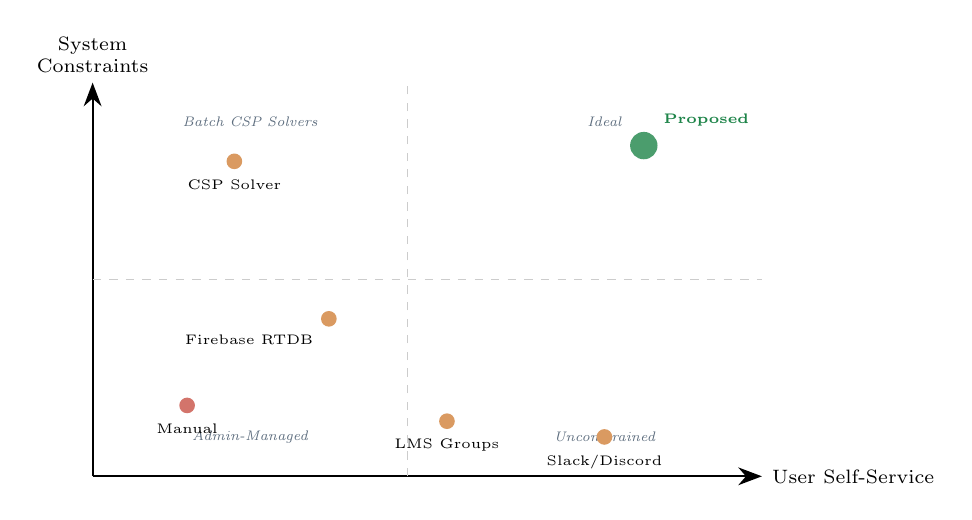
\begin{tikzpicture}[
    every node/.style={font=\small},
    box/.style={draw, rounded corners=4pt, minimum width=2cm, minimum height=1cm, align=center, line width=0.6pt}
]
    % Axes
    \draw[-{Stealth[length=3mm]}, thick] (0,0) -- (8.5,0) node[right, font=\scriptsize] {User Self-Service};
    \draw[-{Stealth[length=3mm]}, thick] (0,0) -- (0,5.0) node[above, font=\scriptsize, align=center] {System\\Constraints};

    % Quadrant labels
    \node[font=\tiny\itshape, color=chartgray] at (2.0, 4.5) {Batch CSP Solvers};
    \node[font=\tiny\itshape, color=chartgray] at (6.5, 4.5) {Ideal};
    \node[font=\tiny\itshape, color=chartgray] at (2.0, 0.5) {Admin-Managed};
    \node[font=\tiny\itshape, color=chartgray] at (6.5, 0.5) {Unconstrained};

    % Existing solutions
    \node[circle, fill=chartred!70, inner sep=2pt, label={[font=\tiny]below:Manual}] at (1.2, 0.9) {};
    \node[circle, fill=chartorange!70, inner sep=2pt, label={[font=\tiny]below:CSP Solver}] at (1.8, 4.0) {};
    \node[circle, fill=chartorange!70, inner sep=2pt, label={[font=\tiny]below:LMS Groups}] at (4.5, 0.7) {};
    \node[circle, fill=chartorange!70, inner sep=2pt, label={[font=\tiny]below:Slack/Discord}] at (6.5, 0.5) {};
    \node[circle, fill=chartorange!70, inner sep=2pt, label={[font=\tiny]below left:Firebase RTDB}] at (3.0, 2.0) {};

    % Our solution
    \node[circle, fill=chartgreen!80, inner sep=3.5pt, label={[font=\tiny\bfseries, color=chartgreen]above right:Proposed}] at (7.0, 4.2) {};

    % Dashed lines for quadrants
    \draw[dashed, gray!40] (4.0, 0) -- (4.0, 5.0);
    \draw[dashed, gray!40] (0, 2.5) -- (8.5, 2.5);
\end{tikzpicture}
\caption{Positioning of web group-formation approaches along user self-service and system constraint enforcement dimensions. Existing solutions cluster in three quadrants; the upper-right quadrant (high self-service + high constraint enforcement) remains unoccupied.}
\label{fig:gap}
\end{figure}

\subsection{Contributions}

This paper makes seven contributions:

\begin{enumerate}[noitemsep,topsep=4pt]
    \item A \textbf{formal constraint model} (Section~\ref{sec:constraints}) with four configurable parameters, feasibility conditions with proof, and a correctness proposition for the two-phase validation algorithm.

    \item A \textbf{two-phase validation algorithm} (Section~\ref{sec:constraints}) that distinguishes hard blocks from soft warnings during iterative group construction, with $O(|T| + |\mathcal{R}|)$ time complexity and server-side re-validation for race-condition protection under concurrent modifications.

    \item A \textbf{six-layer data integrity framework} (Section~\ref{sec:integrity}) that guarantees single-group membership, invite idempotency, duplicate prevention, and cascade cleanup on NoSQL infrastructure without distributed locks or multi-document transactions.

    \item A \textbf{stateless round-robin API key rotation algorithm} (Section~\ref{subsec:roundrobin}) with automatic failover that multiplies the effective throughput of rate-limited external APIs by a factor of~$n$, with $O(1)$ expected and $O(n)$ worst-case key selection.

    \item A \textbf{five-layer defense-in-depth security architecture} (Section~\ref{sec:security}) combining email-based OTP authentication, JWT sessions, database custom tokens, document-level access control, and IP-based sliding-window rate limiting.

    \item A \textbf{three-tier serverless reference implementation} (Section~\ref{sec:architecture}) comprising 8,245~lines of TypeScript across 58~files, with 11~REST API endpoints, 8~NoSQL collections, and real-time event delivery via document-level subscriptions.

    \item A \textbf{production evaluation} (Section~\ref{sec:evaluation}) with 823~users across 7~attribute categories, demonstrating 100\%~constraint satisfaction, zero data integrity violations, sub-second real-time feedback, and linear email-throughput scaling with API keys.
\end{enumerate}

The remainder of this paper is organized as follows. Section~\ref{sec:related} surveys related work across seven research areas. Section~\ref{sec:model} presents the system model and design principles. Section~\ref{sec:constraints} formalizes the constraint model with feasibility and correctness proofs. Section~\ref{sec:architecture} describes the system architecture, including the round-robin API key rotation. Section~\ref{sec:integrity} details the six-layer data integrity framework. Section~\ref{sec:security} presents the security architecture. Section~\ref{sec:evaluation} reports the production evaluation results. Section~\ref{sec:discussion} discusses findings and limitations. Section~\ref{sec:future} outlines future work. Section~\ref{sec:conclusion} concludes.

% ============================================================
\section{Related Work}
\label{sec:related}
% ============================================================

\subsection{Real-Time Web Architectures}

The evolution from polling-based to push-based web architectures has enabled a new class of interactive applications. The WebSocket protocol~\cite{pimentel2012} provides full-duplex communication over a single TCP connection, enabling server-initiated data delivery without the overhead of HTTP long-polling. Lubbers and Greco~\cite{lubbers2010} demonstrate that WebSocket reduces latency by 3:1 and bandwidth by 500:1 compared to HTTP polling for high-frequency data streams. Server-Sent Events (SSE)~\cite{grigorik2013} provide a simpler, unidirectional alternative suitable for scenarios where the server pushes updates to clients without requiring bidirectional communication.

Firebase Firestore~\cite{firebase} implements a document-level subscription model through its \texttt{onSnapshot()} API, which pushes data changes to connected clients whenever the subscribed document is modified. Unlike WebSocket-based architectures that require explicit server-side event emission, Firestore's subscription model is declarative: clients subscribe to document paths, and the infrastructure handles change detection, conflict resolution, and delivery. This model is particularly well-suited for applications where multiple users observe shared state (e.g., group composition) and require immediate visual feedback when that state changes.

However, real-time delivery infrastructure alone does not address the \emph{semantic} challenge of constraint enforcement. Existing real-time web frameworks provide the communication substrate but leave application-level invariants---such as group composition rules, membership uniqueness, and state-machine transition validity---entirely to the application developer. Our work builds on Firestore's real-time capabilities while adding a formal constraint layer and multi-level integrity guarantees.

\subsection{Constraint Satisfaction in Web Systems}

Lappas et al.~\cite{lappas2009} formalize team formation as a constrained optimization problem on social networks and establish its NP-hardness for the general case where both team quality and inter-member communication cost must be optimized simultaneously. Their approximation algorithms provide provable guarantees for offline settings where all candidates are known in advance.

Anagnostopoulos et al.~\cite{anagnostopoulos2012} extend this to \emph{online} settings where members arrive sequentially and assignments are irrevocable---a model closer to self-service web platforms where users register and join groups over extended periods. Their competitive analysis shows that online algorithms achieve ratios within constant factors of offline optima for practical constraint structures.

Wi et al.~\cite{wi2009} apply genetic algorithms to optimize team competency coverage, demonstrating that evolutionary approaches handle complex multi-objective constraints in R\&D settings.

The constraint satisfaction programming (CSP) literature~\cite{rossi2006, kumar1992, tsang1999} provides the formal foundations for constraint modeling, including arc consistency, backtracking search, and constraint propagation. However, CSP solvers operate in batch mode---they compute complete solutions after all variables and constraints are specified---and are not designed for the interactive, incremental constraint evaluation required by real-time web platforms. Our constraint model draws on CSP formalism (parameterized rules, feasibility analysis) while adapting the evaluation strategy for real-time, per-operation validation.

\subsection{NoSQL Data Integrity}

Brewer's CAP theorem~\cite{brewer2000}, formalized by Gilbert and Lynch~\cite{gilbert2002}, establishes that distributed systems cannot simultaneously guarantee consistency, availability, and partition tolerance. NoSQL databases such as Amazon DynamoDB~\cite{decandia2007} and Google Cloud Firestore~\cite{firebase} prioritize availability and partition tolerance, offering eventual consistency~\cite{vogels2009} or strong consistency within bounded scopes (e.g., single-document reads in Firestore).

The absence of multi-document ACID transactions in many NoSQL systems creates a fundamental challenge for web applications that must enforce cross-document invariants. Cattell~\cite{cattell2010} surveys NoSQL data stores and identifies the lack of referential integrity enforcement as a key trade-off. Stonebraker~\cite{stonebraker2010} argues that this trade-off is acceptable for workloads that are partitionable by entity, but problematic for workloads requiring cross-entity consistency.

Chang et al.~\cite{chang2006} describe Bigtable's single-row transaction model, which provides atomicity for operations within a single entity but not across entities. Firestore extends this with single-document atomicity and limited multi-document transactions (up to 500 documents per batch), but cross-collection invariants still require application-level enforcement.

Our six-layer data integrity framework (Section~\ref{sec:integrity}) addresses this gap by implementing invariant enforcement at multiple application levels---UI guards, API-layer validation, and database security rules---providing defense-in-depth integrity without relying on database-level transactions.

\subsection{Serverless Architecture Patterns}

Jonas et al.~\cite{jonas2017} introduce the serverless computing paradigm, arguing that auto-scaling, pay-per-use cloud functions democratize access to scalable infrastructure. The Berkeley view on serverless computing~\cite{jonas2019} identifies key challenges: cold-start latency, limited execution duration, and the absence of persistent local state.

Baldini et al.~\cite{baldini2017} survey serverless computing patterns and identify stateful serverless applications as an open problem. McGrath and Brenner~\cite{mcgrath2017} benchmark serverless function performance across providers, finding that cold-start latencies range from 100ms to several seconds depending on runtime and provider.

Schleier-Smith et al.~\cite{schleier-smith2021} argue that the next phase of serverless computing must address state management, proposing programming models that integrate state into the serverless paradigm.

Our architecture operates within the constraints of current serverless platforms: in-memory state (rate-limit counters) is tolerated as best-effort and resets on cold starts; persistent state resides entirely in the NoSQL database; and API key rotation is stateless modulo a single in-memory counter. This design achieves zero-cost deployment on free tiers while accepting the trade-offs inherent in serverless infrastructure.

\subsection{Rate Limiting and API Key Management}

Rate limiting is a foundational mechanism for protecting web services from abuse and ensuring fair resource allocation. The token bucket and leaky bucket algorithms~\cite{tanenbaum2011} are widely deployed in API gateways and reverse proxies. The IETF has proposed standardized rate-limit response headers~\cite{ietf-ratelimit2024} to communicate quota status to clients.

Raghavan et al.~\cite{raghavan2007} address distributed rate limiting in cloud environments, proposing algorithms that maintain global rate limits across geographically distributed enforcement points. Their work focuses on \emph{incoming} request rate limiting (protecting the server), whereas our round-robin algorithm addresses \emph{outgoing} request rate limiting (operating within external API quotas)---a complementary but distinct problem.

The specific challenge of multiplying effective API capacity through multi-key rotation has received little formal treatment in the literature. Commercial platforms (SendGrid, Brevo, Mailgun) document per-key quotas but do not provide client-side rotation algorithms. Our round-robin approach (Section~\ref{subsec:roundrobin}) formalizes this pattern with complexity analysis and fault-tolerance properties.

\subsection{Self-Service Platforms and Workflow Management}

Self-service web platforms enable end users to perform workflows previously requiring administrator intervention. Van der Aalst et al.~\cite{vanderaalst2003} survey business process management systems, identifying workflow patterns that recur across domains. Harel's statecharts~\cite{harel1987} provide a visual formalism for modeling complex system behavior, including concurrent states and hierarchical decomposition.

Finite state machines (FSMs) are widely used to model entity lifecycle in web applications~\cite{hopcroft1971}. Our system employs FSMs for two critical state transitions: group status (forming $\rightarrow$ full $\rightarrow$ locked) and invitation status (pending $\rightarrow$ approved/rejected/expired). The FSM model ensures that terminal states are immutable and that concurrent transition attempts are handled idempotently.

Bafoutsou and Mentzas~\cite{bafoutsou2002} classify collaborative systems by functionality, identifying group formation, awareness, and communication as core capabilities. Olson and Olson~\cite{olson2000} study distance collaboration, emphasizing the importance of shared awareness of group state---a requirement our real-time subscription architecture directly addresses.

\subsection{Web Application Security}

The OWASP Top Ten~\cite{owasp2021} identifies injection, broken authentication, and cross-site scripting (XSS) as the most critical web application security risks. Barth et al.~\cite{barth2008} provide robust defenses against cross-site request forgery (CSRF), including the \texttt{SameSite} cookie attribute that our implementation employs.

JWT~\cite{jones2015} provides a compact, self-contained token format for session management. Hardt~\cite{hardt2012} defines the OAuth 2.0 framework for delegated authorization. Stuttard and Pinto~\cite{stuttard2011} provide a comprehensive treatment of web application attack vectors and defenses.

Our five-layer security model (Section~\ref{sec:security}) implements defense-in-depth~\cite{owasp2021} with OTP-based authentication~\cite{mraihi2011}, JWT sessions, database-level access control, transport security headers, and IP-based rate limiting. This architecture is designed for environments where institutional single sign-on (SSO) is unavailable---a common constraint in platforms serving users who lack pre-existing organizational credentials.

% ============================================================
\section{System Model}
\label{sec:model}
% ============================================================

\subsection{Design Principles}

The platform is designed around five principles derived from web systems research:

\begin{enumerate}[noitemsep,topsep=4pt]
    \item \textbf{User self-service:} Users initiate group creation, select members, and choose which groups to join---enabling autonomous workflow completion without administrator intervention.
    \item \textbf{Automated constraint enforcement:} Every member addition is validated against configurable composition rules in real time, preventing invalid group configurations at the point of user action rather than through post-hoc administrative review.
    \item \textbf{Progressive guidance:} Soft warnings guide users toward constraint satisfaction during intermediate group-building stages, with hard blocks only at the point of violation or group completion. This design respects human decision-making processes by providing information at the point when it becomes actionable.
    \item \textbf{Data integrity by design:} Duplication prevention, idempotent operations, and cascade cleanup are built into every state transition, not bolted on after the fact. Invariants are enforced at multiple application levels (defense-in-depth).
    \item \textbf{Platform governance:} Gate controls, bulk data management, real-time statistics, and intervention capabilities provide administrative oversight without micromanagement of individual user workflows.
\end{enumerate}

\subsection{Workflow Model}

The group formation process follows four phases (Fig.~\ref{fig:workflow}):

\begin{figure}[htbp]
\centering
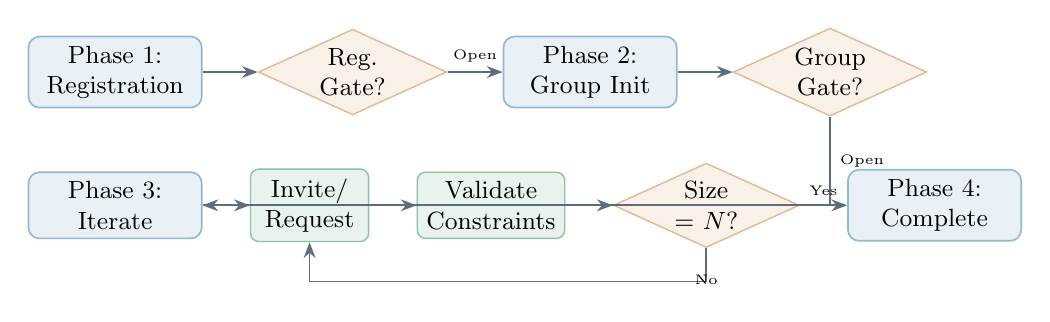
\begin{tikzpicture}[
    node distance=0.5cm and 0.6cm,
    every node/.style={font=\small},
    phase/.style={draw, rounded corners=4pt, minimum width=2.2cm, minimum height=0.8cm, align=center, fill=chartblue!10, draw=chartblue!50, line width=0.6pt},
    gate/.style={draw, diamond, aspect=2.2, minimum width=1.2cm, align=center, fill=chartorange!10, draw=chartorange!50, line width=0.5pt, inner sep=1pt, font=\small},
    act/.style={draw, rounded corners=3pt, minimum width=1.5cm, minimum height=0.6cm, align=center, fill=chartgreen!10, draw=chartgreen!50, line width=0.5pt},
    arrow/.style={-{Stealth[length=2mm]}, draw=chartgray, semithick}
]
    % Phase 1
    \node[phase] (reg) {Phase 1:\\Registration};
    \node[gate, right=0.7cm of reg] (reggate) {Reg.\\Gate?};

    % Phase 2
    \node[phase, right=0.7cm of reggate] (team) {Phase 2:\\Group Init};
    \node[gate, right=0.7cm of team] (teamgate) {Group\\Gate?};

    % Phase 3
    \node[phase, below=0.8cm of reg] (grow) {Phase 3:\\Iterate};
    \node[act, right=0.6cm of grow] (invite) {Invite/\\Request};
    \node[act, right=0.6cm of invite] (validate) {Validate\\Constraints};
    \node[gate, right=0.6cm of validate] (full) {Size\\= $N$?};

    % Phase 4
    \node[phase, right=0.6cm of full] (done) {Phase 4:\\Complete};

    % Arrows
    \draw[arrow] (reg) -- (reggate);
    \draw[arrow] (reggate) -- node[above, font=\tiny] {Open} (team);
    \draw[arrow] (team) -- (teamgate);
    \draw[arrow] (teamgate) |- node[right, near start, font=\tiny] {Open} (grow);
    \draw[arrow] (grow) -- (invite);
    \draw[arrow] (invite) -- (validate);
    \draw[arrow] (validate) -- (full);
    \draw[arrow] (full) -- node[above, font=\tiny] {Yes} (done);
    \draw[arrow] (full) |- node[below, near start, font=\tiny] {No} ([yshift=-0.5cm]invite.south) -- (invite);
\end{tikzpicture}
\caption{Four-phase group formation workflow with administrative gate controls between phases. Phase~3 iterates until the group reaches the required size $N$ with all constraints satisfied.}
\label{fig:workflow}
\end{figure}

\textbf{Phase~1 (Registration):} Users authenticate via email OTP and register on the platform. The system validates user identifiers against an enrollment database using configurable patterns. An admin-controlled registration gate enables phased enrollment.

\textbf{Phase~2 (Group Initiation):} Users create new groups (generating a unique human-readable group code) or browse existing open groups. A separate group formation gate controls when this phase becomes available. The group creator is assigned as the ``group lead'' with invite and management privileges.

\textbf{Phase~3 (Iterative Building):} This is the core formation phase with two parallel interaction modes:
\begin{itemize}[noitemsep,topsep=3pt]
    \item \textbf{Invite mode:} Group leads invite specific users by identifier. The system validates existence, registration status, group membership status, and pending-invite status before creating the invitation.
    \item \textbf{Request mode:} Users browse open groups, view current composition and constraint status, and submit join requests. The system validates membership and pending-request status before creating the request.
\end{itemize}
Every member addition---whether via invite acceptance or request approval---passes through the constraint engine (Section~\ref{sec:constraints}) and the data integrity framework (Section~\ref{sec:integrity}) before being committed to the database.

\textbf{Phase~4 (Completion):} When a group reaches $N$ members with all constraints satisfied, it is marked complete. The full composition validation (Algorithm~\ref{alg:validate}) ensures every constraint is met.

\subsection{Dual-Interaction Model}

A distinctive feature of the platform is its \textbf{dual-interaction model}: group leads actively recruit (invite mode) while unaffiliated users proactively seek groups (browse/request mode). This addresses the ``cold-start problem'' where early-registering users have few groups to browse. Group leads can seed their groups through invitations while simultaneously receiving join requests from browsers.

The browse interface displays each group's current composition, attribute distribution, open slots, and constraint status---enabling informed decision-making. Users can see which groups need members with their attribute category (addressing mandatory representation requirements), creating a marketplace-like dynamic where supply (users) and demand (group slots with specific attribute needs) naturally equilibrate.

\subsection{Platform Governance Layer}

The administrative interface provides three categories of control:
\begin{enumerate}[noitemsep,topsep=4pt]
    \item \textbf{Gate management:} Independent toggles for the registration gate and group formation gate, enabling phased rollouts.
    \item \textbf{Data management:} CSV bulk upload of user enrollment data, individual user management, and group intervention capabilities (remove members, dissolve groups, transfer group lead).
    \item \textbf{Real-time monitoring:} Statistics dashboard showing registration counts, group counts by status, attribute distribution across groups, unaffiliated user counts, and constraint violation alerts.
\end{enumerate}

% ============================================================
\section{Formal Constraint Model}
\label{sec:constraints}
% ============================================================

\subsection{Definitions and Parameters}

\begin{definition}[Group and Attribute Model]
Let $T = \{m_1, m_2, \ldots, m_n\}$ be a group where each member $m_i$ has an attribute category $b(m_i) \in \mathcal{B}$ for a finite set of attribute categories $\mathcal{B}$. The constraint model is parameterized by:
\begin{itemize}[noitemsep,topsep=3pt]
    \item $N \in \mathbb{Z}^+$: Required group size
    \item $K \in \mathbb{Z}^+$: Maximum members from any single attribute category, where $K < N$
    \item $D \in \mathbb{Z}^+$: Minimum number of unique attribute categories represented, where $D \leq |\mathcal{B}|$
    \item $\mathcal{R} \subseteq \mathcal{B}$: Set of attribute categories requiring mandatory representation
\end{itemize}
\end{definition}

We define the following functions over a group $T$:

\textbf{Attribute distribution:}
\begin{equation}
    \delta(T, \beta) = |\{m_i \in T : b(m_i) = \beta\}|
\end{equation}

\textbf{Diversity measure:}
\begin{equation}
    U(T) = |\{\beta \in \mathcal{B} : \delta(T, \beta) > 0\}|
\end{equation}

\textbf{Concentration ratio:}
\begin{equation}
    \gamma(T) = \frac{\max_{\beta \in \mathcal{B}} \delta(T, \beta)}{|T|}
\end{equation}

A group $T$ is \emph{valid} if and only if all four constraints are satisfied:
\begin{align}
    \mathcal{C}_1(T) &: |T| = N \label{eq:c1} \\
    \mathcal{C}_2(T) &: \max_{\beta \in \mathcal{B}} \delta(T, \beta) \leq K \label{eq:c2} \\
    \mathcal{C}_3(T) &: U(T) \geq D \label{eq:c3} \\
    \mathcal{C}_4(T) &: \forall\, \beta \in \mathcal{R},\; \exists\, m_i \in T : b(m_i) = \beta \label{eq:c4}
\end{align}

\begin{equation}
    \text{valid}(T) \iff \mathcal{C}_1 \wedge \mathcal{C}_2 \wedge \mathcal{C}_3 \wedge \mathcal{C}_4
\end{equation}

This four-parameter model is \textbf{domain-agnostic}: any organization can configure $N$, $K$, $D$, $\mathcal{B}$, and $\mathcal{R}$ to match their specific composition policies without code changes.

\subsection{Constraint Feasibility}

Not all parameter combinations produce feasible group configurations. The following theorem establishes necessary and sufficient conditions for the existence of at least one valid group.

\begin{theorem}[Feasibility Conditions]
\label{thm:feasibility}
A valid group $T$ satisfying $\mathcal{C}_1 \wedge \mathcal{C}_2 \wedge \mathcal{C}_3 \wedge \mathcal{C}_4$ exists if and only if:
\begin{align}
    K &\geq \lceil N / |\mathcal{B}| \rceil \label{eq:feas1} \\
    D &\leq \min(N, |\mathcal{B}|) \label{eq:feas2} \\
    |\mathcal{R}| &\leq N \label{eq:feas3} \\
    |\mathcal{R}| &\leq D \label{eq:feas4} \\
    K \cdot |\mathcal{B}| &\geq N \label{eq:feas5}
\end{align}
\end{theorem}

\begin{proof}
\textbf{Necessity.}
(\ref{eq:feas1}): If $K < \lceil N/|\mathcal{B}| \rceil$, then $K \cdot |\mathcal{B}| < N$ by the ceiling property, meaning even distributing maximally across all categories cannot yield $N$ members.
(\ref{eq:feas2}): The diversity measure $U(T) \leq \min(|T|, |\mathcal{B}|) = \min(N, |\mathcal{B}|)$, so $D > \min(N, |\mathcal{B}|)$ makes $\mathcal{C}_3$ unsatisfiable.
(\ref{eq:feas3}): Each required category needs at least one member, so $|\mathcal{R}| > N$ makes $\mathcal{C}_4$ unsatisfiable with only $N$ members.
(\ref{eq:feas4}): If $|\mathcal{R}| > D$, then satisfying $\mathcal{C}_4$ requires at least $|\mathcal{R}|$ unique categories, but $\mathcal{C}_3$ permits only $D < |\mathcal{R}|$, a contradiction.
(\ref{eq:feas5}): This is the total capacity condition: the maximum number of members across all categories must be at least $N$.

\textbf{Sufficiency.}
We construct a valid group. Place one member from each required category $\beta \in \mathcal{R}$ (possible by \ref{eq:feas3}). This contributes $|\mathcal{R}|$ members and $|\mathcal{R}|$ unique categories. If $U < D$, select $D - |\mathcal{R}|$ additional categories from $\mathcal{B} \setminus \mathcal{R}$ (possible since $D \leq |\mathcal{B}|$) and add one member from each. Now $U = D$, and we have $|\mathcal{R}| + (D - |\mathcal{R}|) = D$ members. The remaining $N - D$ members can be distributed across any categories without exceeding $K$ per category (possible by \ref{eq:feas5}). The resulting group satisfies all four constraints.
\end{proof}

The system validates these feasibility conditions at configuration time and alerts administrators to infeasible parameter combinations before any user interaction begins.

\subsection{Two-Phase Validation Algorithm}

The constraint engine implements a two-phase validation strategy.

\textbf{Phase~A: Pre-Addition Validation.} Before every member addition, Algorithm~\ref{alg:canAdd} checks whether adding a candidate would violate any constraint. Hard constraints ($\mathcal{C}_1$, $\mathcal{C}_2$) block immediately. Soft constraints ($\mathcal{C}_3$, $\mathcal{C}_4$) produce warnings during intermediate stages but become hard blocks when adding the $N$-th member.

\begin{algorithm}[htbp]
\caption{Pre-Addition Constraint Validation (\texttt{canAddMember})}
\label{alg:canAdd}
\small
\begin{algorithmic}[1]
\REQUIRE Approved members $T_a$, candidate category $\beta_c$, params $N, K, D, \mathcal{R}$
\ENSURE (valid, errors, warnings)
\STATE $E \gets \emptyset$; $W \gets \emptyset$
\IF{$|T_a| \geq N$}
    \STATE $E$.add(``Group full'')
    \RETURN (false, $E$, $W$)
\ENDIF
\IF{$\delta(T_a, \beta_c) + 1 > K$}
    \STATE $E$.add(``Max $K$ from category $\beta_c$'')
\ENDIF
\IF{$|T_a| + 1 = N$}
    \STATE \COMMENT{Final member: enforce all constraints}
    \STATE $T' \gets T_a \cup \{\text{candidate}\}$
    \IF{$U(T') < D$}
        \STATE $E$.add(``Need $\geq D$ unique categories'')
    \ENDIF
    \FOR{each $\beta \in \mathcal{R}$}
        \IF{$\delta(T', \beta) = 0$}
            \STATE $E$.add(``Need member from category $\beta$'')
        \ENDIF
    \ENDFOR
\ELSIF{$|T_a| + 1 \geq N - 2$}
    \STATE $T' \gets T_a \cup \{\text{candidate}\}$
    \FOR{each $\beta \in \mathcal{R}$}
        \IF{$\delta(T', \beta) = 0$}
            \STATE $s \gets N - |T_a| - 1$
            \STATE $W$.add(``No member from $\beta$ yet; $s$ slots remaining'')
        \ENDIF
    \ENDFOR
\ENDIF
\RETURN ($|E| = 0$, $E$, $W$)
\end{algorithmic}
\end{algorithm}

\textbf{Phase~B: Completion Validation.} When the $N$-th member is added, Algorithm~\ref{alg:validate} enforces all four constraints simultaneously.

\begin{algorithm}[htbp]
\caption{Full Group Composition Validation (\texttt{validateComposition})}
\label{alg:validate}
\small
\begin{algorithmic}[1]
\REQUIRE Group members $T$, params $N, K, D, \mathcal{R}$
\ENSURE (valid, errors)
\STATE $E \gets \emptyset$
\STATE $T_a \gets \{m \in T : m.\text{status} = \text{``approved''}\}$
\IF{$|T_a| \neq N$}
    \STATE $E$.add(``Group size must be $N$'')
\ENDIF
\STATE Compute $\delta(T_a, \beta)$ for all $\beta \in \mathcal{B}$ via hash map
\IF{$\max_\beta \delta(T_a, \beta) > K$}
    \STATE $E$.add(``Max $K$ from any category exceeded'')
\ENDIF
\IF{$U(T_a) < D$}
    \STATE $E$.add(``Need $\geq D$ unique categories'')
\ENDIF
\FOR{each $\beta \in \mathcal{R}$}
    \IF{$\delta(T_a, \beta) = 0$}
        \STATE $E$.add(``Missing required category $\beta$'')
    \ENDIF
\ENDFOR
\RETURN ($|E| = 0$, $E$)
\end{algorithmic}
\end{algorithm}

\begin{proposition}[Correctness]
\label{prop:correctness}
If every member addition passes Algorithm~\ref{alg:canAdd} and the final group passes Algorithm~\ref{alg:validate}, then the resulting group~$T$ satisfies $\text{valid}(T)$.
\end{proposition}

\begin{proof}
Algorithm~\ref{alg:canAdd} enforces $\mathcal{C}_1$ (line~2--4: rejects additions to full groups) and $\mathcal{C}_2$ (line~5--6: rejects additions exceeding the per-category limit~$K$) at every addition. When $|T_a| + 1 = N$, it additionally enforces $\mathcal{C}_3$ (lines~9--10) and $\mathcal{C}_4$ (lines~11--13). Algorithm~\ref{alg:validate} re-checks all four constraints against the final group state. Since both algorithms must pass, $\mathcal{C}_1 \wedge \mathcal{C}_2 \wedge \mathcal{C}_3 \wedge \mathcal{C}_4$ holds for the completed group.
\end{proof}

\subsection{Complexity Analysis}

Both algorithms operate in $O(|T| + |\mathcal{R}|)$ time. The attribute distribution computation requires one pass over the member list ($O(|T|)$) using a hash map, and the mandatory representation check iterates over $\mathcal{R}$ ($O(|\mathcal{R}|)$). Since both $|T| = N$ and $|\mathcal{R}| \leq |\mathcal{B}|$ are small constants in practice (typically $N \leq 10$, $|\mathcal{B}| \leq 15$), the validation executes in constant time---enabling sub-50ms client-side execution.

The space complexity is $O(|\mathcal{B}|)$ for the attribute distribution hash map.

\subsection{Progressive Warning System}

A key design choice is the distinction between \textbf{hard errors} and \textbf{soft warnings}:
\begin{itemize}[noitemsep,topsep=4pt]
    \item \textbf{Hard errors} (group full, category concentration exceeded) block the addition immediately. These constraints are violated at the point of addition and cannot self-correct through subsequent additions.
    \item \textbf{Soft warnings} (insufficient diversity, missing mandatory category) are surfaced as advisory messages during intermediate stages. They become hard errors only when adding the final member, because the group can still satisfy these constraints through subsequent additions.
\end{itemize}

The warning threshold is configurable: in our implementation, warnings activate when $|T_a| + 1 \geq N - 2$ (within 2 slots of completion), providing early notice without disrupting early group building.

\subsection{Race Condition Protection}

In a concurrent multi-user environment, two users may simultaneously attempt to join a nearly-full group. Without protection:
\begin{itemize}[noitemsep,topsep=3pt]
    \item \textbf{Size overflow:} Both additions succeed, producing a group with $N+1$ members.
    \item \textbf{Constraint violation:} Both additions individually pass validation, but their combined effect violates a constraint.
\end{itemize}

We employ a \textbf{read-before-write} pattern: immediately before writing any member addition, the system re-reads the current group document and re-executes \texttt{canAddMember()} against the latest state. This adds one extra database read per operation but guarantees constraint correctness under concurrent modification.

This approach leverages Firestore's strong consistency for single-document reads: reads within the same request observe the most recent committed write. While not equivalent to serializable transactions, this pattern is sufficient for our use case---in the rare case of a genuine race (two writes in the same millisecond), at most one will succeed and the other will be rejected on re-validation.

% ============================================================
\section{System Architecture}
\label{sec:architecture}
% ============================================================

\subsection{Three-Tier Serverless Architecture}

The platform implements a three-tier serverless architecture (Fig.~\ref{fig:architecture}) designed for zero-infrastructure deployment on free-tier cloud services.

\begin{figure}[htbp]
\centering
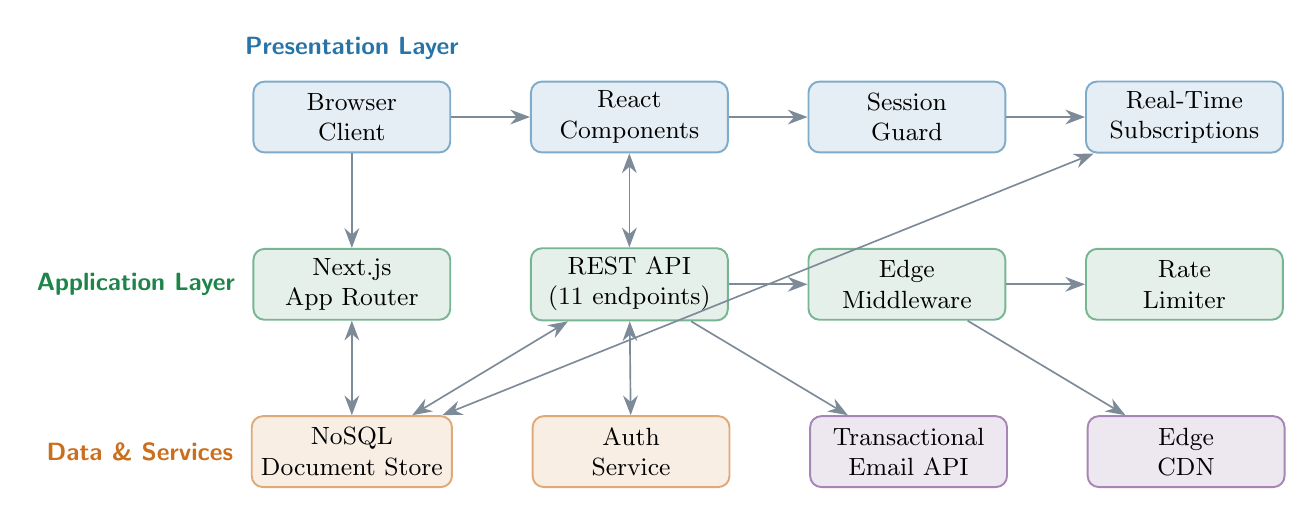
\begin{tikzpicture}[
    node distance=0.8cm and 1.0cm,
    every node/.style={font=\small},
    block/.style={draw, rounded corners=4pt, minimum width=2.5cm, minimum height=0.9cm, align=center, line width=0.7pt},
    client/.style={block, fill=chartblue!12, draw=chartblue!60},
    server/.style={block, fill=chartgreen!12, draw=chartgreen!60},
    db/.style={block, fill=chartorange!12, draw=chartorange!60},
    ext/.style={block, fill=chartpurple!12, draw=chartpurple!60},
    arrow/.style={-{Stealth[length=2.5mm]}, semithick, draw=chartgray!80},
    darrow/.style={{Stealth[length=2.5mm]}-{Stealth[length=2.5mm]}, semithick, draw=chartgray!80},
    lbl/.style={font=\small\bfseries\sffamily}
]
    \node[client] (browser) {Browser\\Client};
    \node[client, right=of browser] (react) {React\\Components};
    \node[client, right=of react] (session) {Session\\Guard};
    \node[client, right=of session] (notif) {Real-Time\\Subscriptions};

    \node[server, below=1.2cm of browser] (nextjs) {Next.js\\App Router};
    \node[server, right=of nextjs] (api) {REST API\\(11 endpoints)};
    \node[server, right=of api] (mw) {Edge\\Middleware};
    \node[server, right=of mw] (rate) {Rate\\Limiter};

    \node[db, below=1.2cm of nextjs] (firestore) {NoSQL\\Document Store};
    \node[db, right=of firestore] (auth) {Auth\\Service};
    \node[ext, right=of auth] (email) {Transactional\\Email API};
    \node[ext, right=of email] (cdn) {Edge\\CDN};

    \draw[arrow] (browser) -- (react);
    \draw[arrow] (react) -- (session);
    \draw[arrow] (session) -- (notif);
    \draw[arrow] (browser) -- (nextjs);
    \draw[darrow] (react) -- (api);
    \draw[arrow] (api) -- (mw);
    \draw[arrow] (mw) -- (rate);
    \draw[darrow] (nextjs) -- (firestore);
    \draw[darrow] (api) -- (firestore);
    \draw[darrow] (api) -- (auth);
    \draw[arrow] (api) -- (email);
    \draw[arrow] (mw) -- (cdn);
    \draw[darrow] (notif) -- (firestore);

    \node[lbl, color=chartblue, above=0.15cm of browser] {Presentation Layer};
    \node[lbl, color=chartgreen, left=0.1cm of nextjs, anchor=east] {Application Layer};
    \node[lbl, color=chartorange, left=0.1cm of firestore, anchor=east] {Data \& Services};
\end{tikzpicture}
\caption{Three-tier serverless architecture with real-time document subscriptions enabling instant constraint feedback and notifications.}
\label{fig:architecture}
\end{figure}

The architecture is technology-agnostic in principle; our reference implementation uses Next.js~\cite{nextjs}, Firebase Firestore~\cite{firebase}, and Brevo Email API, but any equivalent stack could implement the same model.

\textbf{Presentation Layer.} The client is a React single-page application rendered via server-side rendering (SSR) for initial page loads and client-side navigation thereafter. The SessionGuard component implements a three-phase authentication check: (1)~local storage for cached session state, (2)~JWT and database token initialization, and (3)~document verification against the registration database. Real-time notifications use the document store's subscription API with an initialization flag to suppress notification alerts during initial data hydration.

\textbf{Application Layer.} The App Router handles 11 REST API endpoints (Table~\ref{tab:endpoints}), each implementing input validation, authentication verification, business logic, and response formatting. Edge middleware intercepts all API requests for origin verification, security header injection, and route protection. The rate limiter operates at the IP level with configurable sliding windows.

\textbf{Data Layer.} The NoSQL document store provides real-time subscriptions. The authentication service provides custom token infrastructure for client-side database access. External services include the transactional email API (with multi-key round-robin) and the edge CDN for static asset delivery.

\subsection{API Design}

Table~\ref{tab:endpoints} lists all 11 REST endpoints with their methods and purposes.

\begin{table}[htbp]
\centering
\caption{REST API Endpoints}
\label{tab:endpoints}
\small
\renewcommand{\arraystretch}{1.15}
\begin{tabular}{@{}lll@{}}
\toprule
\textbf{Endpoint} & \textbf{Method} & \textbf{Purpose} \\
\midrule
\texttt{/auth/send-otp} & POST & Send OTP via email \\
\texttt{/auth/verify-otp} & POST & Verify OTP, issue JWT \\
\texttt{/auth/lookup-usn} & POST & Validate user identifier \\
\texttt{/auth/logout} & POST & Clear session \\
\texttt{/auth/firebase-token} & GET & Refresh database token \\
\texttt{/admin/upload-csv} & POST & Bulk data import \\
\texttt{/admin/config} & GET/POST & System configuration \\
\texttt{/admin/students/:id} & PUT/DEL & Individual user mgmt. \\
\texttt{/admin/reset-database} & POST & Database reset (admin) \\
\texttt{/notify/email} & POST & Email notifications \\
\bottomrule
\end{tabular}
\end{table}

Each endpoint follows a consistent request/response pattern:
\begin{itemize}[noitemsep,topsep=3pt]
    \item \textbf{Input validation:} Request bodies are validated for required fields and type correctness before any business logic executes.
    \item \textbf{Authentication:} Protected endpoints verify JWT session tokens (user endpoints) or admin ID tokens (admin endpoints).
    \item \textbf{Rate limiting:} Abuse-sensitive endpoints (OTP send/verify) enforce per-IP sliding-window rate limits.
    \item \textbf{Response format:} All responses use JSON with a consistent \texttt{\{success, error, data\}} structure.
\end{itemize}

\subsection{NoSQL Schema Design}

The database uses 8 collections (Table~\ref{tab:collections}). A key design decision is \textbf{embedding member arrays within group documents} rather than using normalized junction collections. This denormalized design enables:

\begin{itemize}[noitemsep,topsep=4pt]
    \item \textbf{Single-document reads:} Complete group state (all members, attributes, statuses) is retrieved in one database read, critical for real-time constraint validation.
    \item \textbf{Atomic member operations:} Adding or removing a member is an atomic update to a single document, preventing partial-state issues.
    \item \textbf{Efficient subscriptions:} Real-time listeners subscribe to one document per group, reducing subscription overhead.
    \item \textbf{Natural deduplication:} Member arrays are mapped by user identifier, preventing duplicate entries at the data model level.
\end{itemize}

\begin{table}[htbp]
\centering
\caption{Database Collections and Document Schemas}
\label{tab:collections}
\small
\renewcommand{\arraystretch}{1.15}
\begin{tabular}{@{}lp{2cm}p{5.5cm}@{}}
\toprule
\textbf{Collection} & \textbf{Document Key} & \textbf{Schema Fields} \\
\midrule
\texttt{users} & User ID & name, email, phone, category, section, importedAt \\
\texttt{registrations} & User ID & name, email, category, section, groupId (FK), groupRole, registeredAt \\
\texttt{groups} & Group code & name, leadId, members[] (embedded), memberCount, status (FSM), categoryDistribution, isPublic, timestamps \\
\texttt{invites} & Invite code & type (invite|request), groupId, fromId, toId, status (FSM), timestamps \\
\texttt{notifications} & Auto-generated & userId, type (10 event types), title, message, groupId, fromId, read, createdAt \\
\texttt{config} & Singleton & registrationsOpen, groupFormationOpen, maxGroupSize, minCategories, maxSameCategory, requiredCategories \\
\texttt{otp\_codes} & Auto-generated & email, otp, expiresAt, used, attempts, createdAt \\
\texttt{admins} & Email hash & Admin whitelist \\
\bottomrule
\end{tabular}
\end{table}

The \texttt{groups} collection embeds member arrays with the following per-member fields: user identifier, name, attribute category, section, status (\texttt{approved} | \texttt{pending\_invite} | \texttt{pending\_request}), and join timestamp. The \texttt{categoryDistribution} field is a denormalized map (category $\rightarrow$ count) maintained atomically with member operations, enabling $O(1)$ constraint checks without iterating the member array.

\subsection{Real-Time Event Architecture}

The platform implements real-time data delivery through two complementary mechanisms:

\textbf{Document subscriptions.} Client-side components subscribe to specific documents (the user's registration document, the user's group document) and receive push updates whenever these documents change. This enables instant UI updates when a member joins, an invitation is accepted, or the group status transitions.

\textbf{Query-based polling.} For aggregate views (browse page, admin dashboard), the platform uses periodic query-based data fetching rather than document subscriptions, as subscribing to all group documents would create excessive subscription overhead. A \texttt{useCallback}-based fetch pattern with session synchronization ensures data consistency:

\begin{lstlisting}[language={}, caption={Session synchronization pattern}, label={lst:sessionsync}]
const fetchData = useCallback(async () => {
  // Re-fetch registration to fix stale session
  const regDoc = await getDoc(
    doc(db, "registrations", session.userId)
  );
  if (regDoc.exists()) {
    const data = regDoc.data();
    // Sync session if groupId changed
    if (data.groupId !== session.groupId) {
      updateSession(data.groupId, data.groupRole);
    }
  }
  // Fetch group and pending invites...
}, [session.userId]);
\end{lstlisting}

The notification system delivers events through two channels simultaneously: (1)~in-app real-time delivery via document subscriptions with an \texttt{isInitialLoad} flag to distinguish between initial data hydration and genuine new notifications, and (2)~email notifications via the transactional email API for offline awareness.

\subsection{Round-Robin API Key Rotation}
\label{subsec:roundrobin}

Free-tier transactional email services typically limit daily volume (e.g., 300~emails/day per API key). For platforms with 500+ users, this is insufficient during peak registration periods. We present a stateless round-robin algorithm with automatic failover that multiplies effective capacity by a factor of~$n$ (the number of API keys).

\begin{algorithm}[htbp]
\caption{Round-Robin API Key Rotation with Failover}
\label{alg:roundrobin}
\small
\begin{algorithmic}[1]
\REQUIRE Recipient email, subject, body
\ENSURE Email sent successfully or all keys exhausted
\STATE $\mathit{creds} \gets \texttt{parseCredentials}(\texttt{env.MULTI\_KEYS})$
\IF{$|\mathit{creds}| = 0$}
    \STATE \textbf{throw} ``No API keys configured''
\ENDIF
\STATE $\mathit{startIdx} \gets \mathit{rrIndex} \bmod |\mathit{creds}|$ \COMMENT{Round-robin selection}
\STATE $\mathit{rrIndex} \gets \mathit{rrIndex} + 1$ \COMMENT{Advance for next call}
\FOR{$\mathit{attempt} \gets 0$ \TO $|\mathit{creds}| - 1$}
    \STATE $\mathit{idx} \gets (\mathit{startIdx} + \mathit{attempt}) \bmod |\mathit{creds}|$
    \STATE $\mathit{result} \gets \texttt{sendEmail}(\mathit{creds}[\mathit{idx}], \text{recipient}, \text{subject}, \text{body})$
    \IF{$\mathit{result}.\text{ok}$}
        \RETURN \COMMENT{Success}
    \ENDIF
    \IF{$\mathit{result}.\text{status} \in \{429, 401, 500\}$}
        \STATE \textbf{continue} \COMMENT{Try next key}
    \ENDIF
\ENDFOR
\STATE \textbf{throw} ``All API keys exhausted''
\end{algorithmic}
\end{algorithm}

The algorithm has several important properties:

\textbf{Load distribution.} The round-robin counter ensures that successive requests use different API keys, distributing load evenly across all $n$ keys. Over $m$ requests, each key receives approximately $m/n$ requests, achieving near-optimal load balancing.

\textbf{Capacity multiplication.} With $n$ API keys each supporting $Q$ requests per day, the total capacity is $nQ$. For our deployment with $n = 3$ keys and $Q = 300$, the effective capacity is 900~emails/day.

\textbf{Automatic failover.} If a key returns an error (HTTP 429 rate-limited, 401 unauthorized, or 500 server error), the algorithm advances to the next key without manual intervention. In the worst case, all $n$ keys are attempted before failure.

\textbf{Statelessness.} The only state is the in-memory round-robin counter, which resets on process restart. This is acceptable because the counter's purpose is load balancing, not correctness---a reset simply means the next few requests may not be perfectly distributed, but no emails are lost or duplicated.

\textbf{Complexity.} The expected-case time complexity is $O(1)$ (the first key succeeds). The worst-case complexity is $O(n)$ (all keys are tried before success or failure). Space complexity is $O(n)$ for the credential array.

\textbf{Generalizability.} The algorithm is not specific to email services. It applies to any rate-limited external API where the client possesses multiple credentials: SMS verification services, payment gateways, geolocation APIs, or any service imposing per-key quotas.

The multi-key configuration uses a compact environment variable format: \texttt{KEY1:SENDER1,KEY2:SENDER2,...}, parsed at startup into a credential array. This enables deployment-time configuration without code changes.

\subsection{Unambiguous ID Generation}

Group codes and invite codes are generated using a character set designed to prevent visual ambiguity:

\begin{center}
\texttt{ABCDEFGHJKLMNPQRSTUVWXYZ23456789}
\end{center}

This 30-character alphabet excludes five commonly confused characters: \texttt{I}/\texttt{1}/\texttt{l}, \texttt{O}/\texttt{0}. Group codes follow the format \texttt{TEAM-XXXX} ($30^4 = 810{,}000$ combinations) and invite codes follow \texttt{INV-XXXXXX} ($30^6 \approx 729$ million combinations), providing sufficient uniqueness for institutional-scale deployments while remaining easy to communicate verbally.

The design is stateless---no sequence counters or coordination is required---and collision probability is negligible for the expected deployment sizes. For a deployment with 200 groups, the birthday-paradox collision probability for 4-character codes is approximately $200^2 / (2 \times 810{,}000) \approx 2.5\%$, mitigated by checking for existing codes before assignment.

% ============================================================
\section{Data Integrity Framework}
\label{sec:integrity}
% ============================================================

A critical challenge in self-service web platforms is \textbf{preventing data duplication and enforcing cross-document invariants} without relying on multi-document transactions. When hundreds of users concurrently create groups, send invitations, and process join requests, numerous integrity violations can occur. Our system implements a \textbf{six-layer data integrity framework} (Fig.~\ref{fig:dupflow}).

\begin{figure}[htbp]
\centering
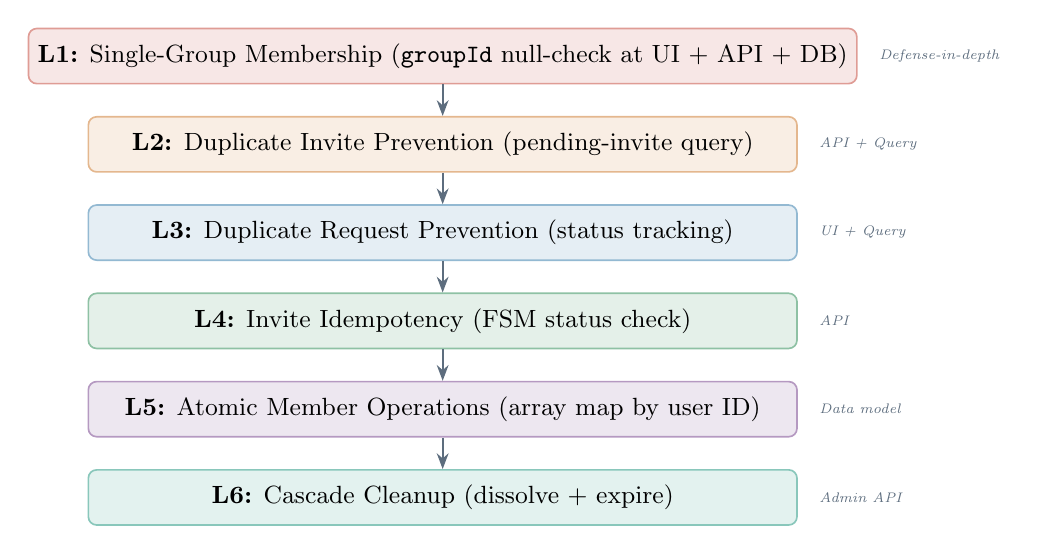
\begin{tikzpicture}[
    node distance=0.4cm,
    every node/.style={font=\small},
    layer/.style={draw, rounded corners=3pt, minimum width=9cm, minimum height=0.7cm, align=center, line width=0.6pt}
]
    \node[layer, fill=chartred!12, draw=chartred!50] (l1) {\textbf{L1:} Single-Group Membership (\texttt{groupId} null-check at UI + API + DB)};
    \node[layer, fill=chartorange!12, draw=chartorange!50, below=of l1] (l2) {\textbf{L2:} Duplicate Invite Prevention (pending-invite query)};
    \node[layer, fill=chartblue!12, draw=chartblue!50, below=of l2] (l3) {\textbf{L3:} Duplicate Request Prevention (status tracking)};
    \node[layer, fill=chartgreen!12, draw=chartgreen!50, below=of l3] (l4) {\textbf{L4:} Invite Idempotency (FSM status check)};
    \node[layer, fill=chartpurple!12, draw=chartpurple!50, below=of l4] (l5) {\textbf{L5:} Atomic Member Operations (array map by user ID)};
    \node[layer, fill=chartteal!12, draw=chartteal!50, below=of l5] (l6) {\textbf{L6:} Cascade Cleanup (dissolve + expire)};

    \draw[-{Stealth[length=2mm]}, semithick, chartgray] (l1) -- (l2);
    \draw[-{Stealth[length=2mm]}, semithick, chartgray] (l2) -- (l3);
    \draw[-{Stealth[length=2mm]}, semithick, chartgray] (l3) -- (l4);
    \draw[-{Stealth[length=2mm]}, semithick, chartgray] (l4) -- (l5);
    \draw[-{Stealth[length=2mm]}, semithick, chartgray] (l5) -- (l6);

    \node[font=\tiny\itshape, color=chartgray, right=0.15cm of l1] {Defense-in-depth};
    \node[font=\tiny\itshape, color=chartgray, right=0.15cm of l2] {API + Query};
    \node[font=\tiny\itshape, color=chartgray, right=0.15cm of l3] {UI + Query};
    \node[font=\tiny\itshape, color=chartgray, right=0.15cm of l4] {API};
    \node[font=\tiny\itshape, color=chartgray, right=0.15cm of l5] {Data model};
    \node[font=\tiny\itshape, color=chartgray, right=0.15cm of l6] {Admin API};
\end{tikzpicture}
\caption{Six-layer data integrity framework. Each layer prevents a specific class of data integrity violation.}
\label{fig:dupflow}
\end{figure}

We now define the formal invariants and describe the enforcement mechanisms for each layer.

\subsection{L1: Single-Group Membership Enforcement}

\begin{definition}[Single-Membership Invariant]
For all users $u$ in the system, $u$ is assigned to at most one group at any time:
\begin{equation}
    \forall u \in \mathcal{U},\; |\{g \in \mathcal{G} : u \in g.\text{members} \wedge u.\text{status} = \text{approved}\}| \leq 1
\end{equation}
\end{definition}

This invariant is enforced at \textbf{three independent levels}:
\begin{enumerate}[noitemsep,topsep=3pt]
    \item \textbf{UI guards:} Client-side components conditionally render ``already assigned'' messages and disable join/create buttons when the user's \texttt{groupId} is non-null.
    \item \textbf{API validation:} The application logic checks the target user's registration document and rejects operations if \texttt{groupId} is set.
    \item \textbf{Database rules:} Document-level security rules restrict \texttt{groupId} updates to the user themselves or a verified group lead of the user's group.
\end{enumerate}

This defense-in-depth approach ensures that even if client-side validation is bypassed (e.g., via browser developer tools), the server-side and database-level checks reject unauthorized membership changes.

\subsection{L2: Duplicate Invite Prevention}

Before a group lead issues an invitation, the system executes three sequential checks:
\begin{enumerate}[noitemsep,topsep=3pt]
    \item \textbf{Existing member check:} Verifies the target is not already in the group's member array.
    \item \textbf{Pending invite check:} Queries the \texttt{invites} collection for any document matching \texttt{(toId, groupId, type=``invite'', status=``pending'')}. Rejects if a pending invite exists.
    \item \textbf{Cross-group check:} Reads the target's registration document and verifies \texttt{groupId} is null.
\end{enumerate}

\subsection{L3: Duplicate Join-Request Prevention}

Symmetrically, when a user requests to join a group, the system queries for any existing document matching \texttt{(fromId, groupId, type=``request'', status=``pending'')}. The browse UI maintains three visual states per group card: default (``Request to Join'' enabled), pending (``Request Pending'' disabled), and rejected (``Request Declined'' with visual indicator).

\subsection{L4: Invite Idempotency}

Each invite document transitions through a finite state machine (Fig.~\ref{fig:invitefsm}):

\begin{figure}[htbp]
\centering
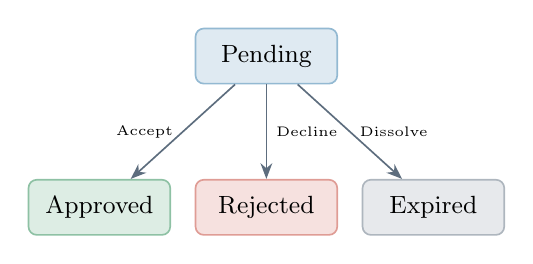
\begin{tikzpicture}[
    node distance=1.8cm,
    every node/.style={font=\small},
    state/.style={draw, rounded corners=3pt, minimum width=1.8cm, minimum height=0.7cm, align=center, line width=0.6pt},
    arrow/.style={-{Stealth[length=2mm]}, semithick, draw=chartgray}
]
    \node[state, fill=chartblue!15, draw=chartblue!50] (pending) {Pending};
    \node[state, fill=chartgreen!15, draw=chartgreen!50, below left=1.2cm and 0.3cm of pending] (approved) {Approved};
    \node[state, fill=chartred!15, draw=chartred!50, below=1.2cm of pending] (rejected) {Rejected};
    \node[state, fill=chartgray!15, draw=chartgray!50, below right=1.2cm and 0.3cm of pending] (expired) {Expired};

    \draw[arrow] (pending) -- node[left, font=\tiny] {Accept} (approved);
    \draw[arrow] (pending) -- node[right, font=\tiny] {Decline} (rejected);
    \draw[arrow] (pending) -- node[right, font=\tiny] {Dissolve} (expired);
\end{tikzpicture}
\caption{Invite status FSM. Terminal states (approved, rejected, expired) are immutable---no further transitions are permitted.}
\label{fig:invitefsm}
\end{figure}

Once an invite leaves the \texttt{pending} state, it cannot be re-processed. The response handler verifies the current status before any action, returning an error for non-pending invites. This guarantees that concurrent acceptance attempts (e.g., clicking ``Accept'' in two browser tabs) cannot result in a user being added twice.

\subsection{L5: Atomic Member-List Operations}

Group member arrays use \textbf{map operations} (not append) for all modifications:
\begin{itemize}[noitemsep,topsep=3pt]
    \item \textbf{Member approval:} Maps over the array, updating the matching user ID entry's status. If the ID is not found, the operation fails.
    \item \textbf{Member removal:} Filters the array to exclude the matching user ID.
    \item \textbf{Invariant:} At most one array entry exists per user ID at any time.
\end{itemize}

\subsection{L6: Cascade Cleanup on Group Dissolution}

When a group is dissolved, the system performs cascade cleanup:
\begin{enumerate}[noitemsep,topsep=3pt]
    \item All approved members have their \texttt{groupId} and \texttt{groupRole} reset to null.
    \item All pending invites and requests are marked as \texttt{expired}.
    \item The group document status is updated to ``dissolved.''
    \item Notification documents are created for all affected members.
\end{enumerate}

Without cascade cleanup, dissolved groups leave \textbf{orphaned state}: users whose registrations still reference a deleted group cannot join new groups because L1 sees a non-null \texttt{groupId}.

\subsection{Comparison with ACID Properties}

Table~\ref{tab:acid} compares the integrity guarantees of our framework with those provided by traditional ACID transactions in relational databases.

\begin{table}[htbp]
\centering
\caption{Comparison of Integrity Guarantees: ACID vs.\ Six-Layer Framework}
\label{tab:acid}
\small
\renewcommand{\arraystretch}{1.15}
\begin{tabular}{@{}p{2.5cm}p{3.5cm}p{3.5cm}@{}}
\toprule
\textbf{Property} & \textbf{ACID (RDBMS)} & \textbf{Six-Layer (NoSQL)} \\
\midrule
Atomicity & Multi-row transactions & Single-document atomic updates (L5) \\
Consistency & Referential integrity constraints & Application-level invariant checks (L1--L4) \\
Isolation & Serializable/snapshot isolation & Read-before-write + FSM idempotency (L4) \\
Durability & Write-ahead log & Firestore persistence guarantees \\
\midrule
Cross-entity invariants & Foreign key constraints & Defense-in-depth at UI + API + DB (L1) \\
Cascade operations & ON DELETE CASCADE & Application-level cascade cleanup (L6) \\
\bottomrule
\end{tabular}
\end{table}

The six-layer framework achieves comparable integrity guarantees to ACID transactions for the specific invariants required by self-service group formation, without the scalability trade-offs of distributed multi-document transactions.

\subsection{Integrity Framework Summary}

Table~\ref{tab:duplication} summarizes the complete framework with enforcement mechanisms.

\begin{table}[htbp]
\centering
\caption{Data Integrity Invariants and Enforcement Mechanisms}
\label{tab:duplication}
\small
\renewcommand{\arraystretch}{1.15}
\begin{tabular}{@{}p{3cm}p{2cm}p{4.5cm}@{}}
\toprule
\textbf{Invariant} & \textbf{Layers} & \textbf{Enforcement Mechanism} \\
\midrule
Single-group membership & UI + API + DB & \texttt{groupId} null-check at 3 levels \\
No duplicate invites & API + Query & Pending-invite query + member check \\
No duplicate requests & UI + Query & Pending-request query + status tracking \\
Invite idempotency & API & FSM status check before transition \\
No duplicate members & Data model & Array map (not append) keyed by ID \\
Cascade on dissolve & Admin API & Bulk reset + invite expiration \\
\bottomrule
\end{tabular}
\end{table}

% ============================================================
\section{Security Architecture}
\label{sec:security}
% ============================================================

The security architecture implements a five-layer defense-in-depth model (Fig.~\ref{fig:security}), designed for environments where users lack pre-existing SSO credentials.

\begin{figure}[htbp]
\centering
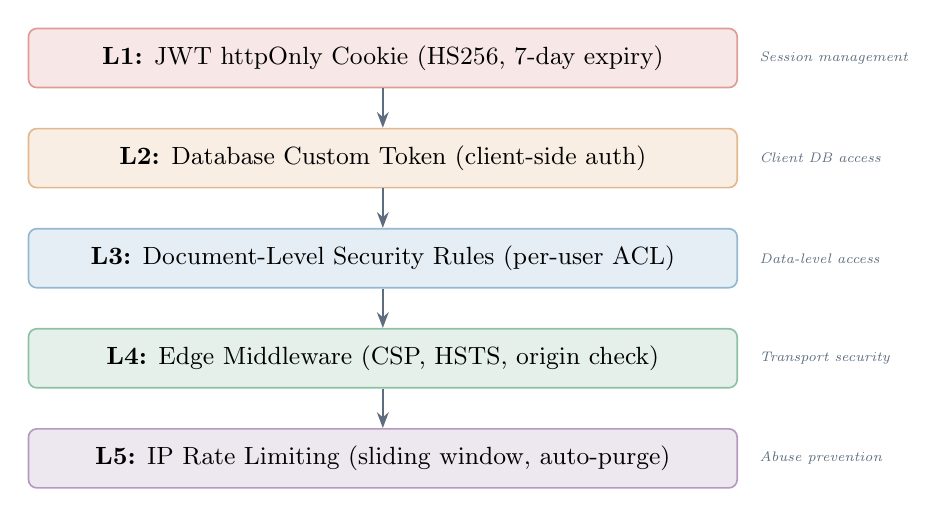
\begin{tikzpicture}[
    node distance=0.5cm,
    every node/.style={font=\small},
    layer/.style={draw, rounded corners=3pt, minimum width=9cm, minimum height=0.75cm, align=center, line width=0.6pt}
]
    \node[layer, fill=chartred!12, draw=chartred!50] (l1) {\textbf{L1:} JWT httpOnly Cookie (HS256, 7-day expiry)};
    \node[layer, fill=chartorange!12, draw=chartorange!50, below=of l1] (l2) {\textbf{L2:} Database Custom Token (client-side auth)};
    \node[layer, fill=chartblue!12, draw=chartblue!50, below=of l2] (l3) {\textbf{L3:} Document-Level Security Rules (per-user ACL)};
    \node[layer, fill=chartgreen!12, draw=chartgreen!50, below=of l3] (l4) {\textbf{L4:} Edge Middleware (CSP, HSTS, origin check)};
    \node[layer, fill=chartpurple!12, draw=chartpurple!50, below=of l4] (l5) {\textbf{L5:} IP Rate Limiting (sliding window, auto-purge)};

    \draw[-{Stealth[length=2mm]}, semithick, chartgray] (l1) -- (l2);
    \draw[-{Stealth[length=2mm]}, semithick, chartgray] (l2) -- (l3);
    \draw[-{Stealth[length=2mm]}, semithick, chartgray] (l3) -- (l4);
    \draw[-{Stealth[length=2mm]}, semithick, chartgray] (l4) -- (l5);

    \node[font=\tiny\itshape, color=chartgray, right=0.15cm of l1] {Session management};
    \node[font=\tiny\itshape, color=chartgray, right=0.15cm of l2] {Client DB access};
    \node[font=\tiny\itshape, color=chartgray, right=0.15cm of l3] {Data-level access};
    \node[font=\tiny\itshape, color=chartgray, right=0.15cm of l4] {Transport security};
    \node[font=\tiny\itshape, color=chartgray, right=0.15cm of l5] {Abuse prevention};
\end{tikzpicture}
\caption{Five-layer defense-in-depth security model. Each layer provides independent protection; compromise of any single layer does not breach the system.}
\label{fig:security}
\end{figure}

\subsection{Layer 1: JWT Session Management}

Upon successful OTP verification, the server issues a JWT~\cite{jones2015} signed with HS256. The token is stored as an \texttt{httpOnly}, \texttt{Secure}, \texttt{SameSite=Lax} cookie with a 7-day expiry. The \texttt{httpOnly} flag prevents JavaScript access, mitigating XSS token theft. The \texttt{SameSite} flag prevents CSRF attacks~\cite{barth2008}.

The JWT payload contains the user's identifier, name, email, attribute category, and current group assignment---enabling client-side rendering of personalized UI without additional database reads.

\subsection{Layer 2: Database Custom Token}

The verification endpoint generates a database custom token using the server-side admin SDK. This token enables direct client-to-database communication through the database's native authentication system, providing real-time subscriptions without routing all reads through the API layer.

\subsection{Layer 3: Document-Level Security Rules}

Database security rules enforce per-document access control:
\begin{lstlisting}[language={}, caption={Document-level security rules (excerpt)}, label={lst:rules}]
match /registrations/{userId} {
  allow read: if request.auth != null;
  allow create: if request.auth != null
    && request.auth.uid == userId;
  allow update: if request.auth != null
    && (request.auth.uid == userId
    || isGroupLead(resource.data.groupId));
}
match /otp_codes/{doc} {
  allow read, write: if false; // server-only
}
\end{lstlisting}

Key rules: users can only modify their own registration documents (except group leads updating group-related fields for their members); OTP codes are completely inaccessible from clients.

\subsection{Layer 4: Edge Middleware}

The edge middleware intercepts all requests matching protected route patterns and applies:
\begin{itemize}[noitemsep,topsep=4pt]
    \item \textbf{Route protection:} Dashboard and group creation routes require valid JWT; unauthenticated users are redirected to the registration page.
    \item \textbf{Origin verification:} API routes verify the \texttt{Origin} header against an allowlist of permitted origins, preventing unauthorized cross-origin access.
    \item \textbf{Security headers:} Every response includes Content-Security-Policy (restricting script sources and connect destinations), X-Frame-Options (DENY), X-Content-Type-Options (nosniff), Referrer-Policy, Permissions-Policy, and Strict-Transport-Security (HSTS with 1-year max-age)~\cite{owasp2021}.
\end{itemize}

\subsection{Layer 5: IP-Based Sliding-Window Rate Limiting}

The rate limiter implements a sliding window algorithm with per-endpoint configuration:

\begin{table}[htbp]
\centering
\caption{Rate Limiting Configuration}
\label{tab:ratelimit}
\small
\renewcommand{\arraystretch}{1.15}
\begin{tabular}{@{}lll@{}}
\toprule
\textbf{Target} & \textbf{Limit} & \textbf{Window} \\
\midrule
OTP send per IP & 5 requests & 15 min \\
OTP verify per IP & 10 attempts & 15 min \\
Per-code incorrect attempts & 5 attempts & Code lifetime \\
Per-email OTP cooldown & 1 OTP & 60 sec \\
\bottomrule
\end{tabular}
\end{table}

The implementation stores timestamps in an in-memory map with a 5-minute auto-purge cycle. IP extraction follows a priority chain: the platform's trusted forwarded header, then \texttt{x-real-ip}, then the connection's remote address.

\begin{lstlisting}[language={}, caption={Sliding-window rate limiter}, label={lst:ratelimit}]
function rateLimit(ip, action, max, windowMs) {
  const key = `${ip}:${action}`;
  const now = Date.now();
  const entry = store.get(key) || { timestamps: [] };
  // Filter to timestamps within window
  entry.timestamps = entry.timestamps
    .filter(t => now - t < windowMs);
  if (entry.timestamps.length >= max) {
    return { allowed: false,
      retryAfterMs: windowMs - (now - entry.timestamps[0])
    };
  }
  entry.timestamps.push(now);
  store.set(key, entry);
  return { allowed: true, retryAfterMs: 0 };
}
\end{lstlisting}

\subsection{Threat Model}

Table~\ref{tab:threats} summarizes the threat model and corresponding mitigations.

\begin{table}[htbp]
\centering
\caption{Threat Model and Mitigations}
\label{tab:threats}
\small
\renewcommand{\arraystretch}{1.15}
\begin{tabular}{@{}p{2.8cm}p{1.5cm}p{5cm}@{}}
\toprule
\textbf{Threat} & \textbf{Layer(s)} & \textbf{Mitigation} \\
\midrule
Session hijacking & L1 & httpOnly + Secure + SameSite cookies \\
XSS token theft & L1, L4 & httpOnly prevents JS access; CSP restricts script sources \\
CSRF & L1, L4 & SameSite cookie; origin verification \\
Brute-force OTP & L5 & 5 attempts/code; 5 sends/IP/15min \\
Direct DB manipulation & L2, L3 & Custom token auth; per-document rules \\
Clickjacking & L4 & X-Frame-Options: DENY \\
MIME sniffing & L4 & X-Content-Type-Options: nosniff \\
Replay attack & L1 & JWT expiration (7 days) \\
Unauthorized API access & L4 & Origin allowlist verification \\
\bottomrule
\end{tabular}
\end{table}

\subsection{OTP Authentication Flow}

The email OTP authentication~\cite{mraihi2011} follows a six-step flow:
\begin{enumerate}[noitemsep,topsep=3pt]
    \item User enters their email address.
    \item System validates the email exists in the enrollment database.
    \item System generates a 6-digit OTP, stores it with a 10-minute TTL and 5-attempt limit.
    \item System sends the OTP via the transactional email API with round-robin key rotation (Algorithm~\ref{alg:roundrobin}).
    \item User enters the OTP within the validity window.
    \item System verifies the OTP, issues a JWT cookie and database custom token, and creates/updates the registration document.
\end{enumerate}

The per-code attempt limit (5) prevents brute-force attacks on the 6-digit code space ($10^6 = 1{,}000{,}000$ combinations). With 5 attempts, the probability of a successful brute-force attack is $5/10^6 = 0.0005\%$.

% ============================================================
\section{Evaluation}
\label{sec:evaluation}
% ============================================================

\subsection{Deployment Setup}

The platform was deployed in production serving 823~users across 7~attribute categories (Table~\ref{tab:categories}). Groups of exactly 6~members were required with the following constraint configuration:
\begin{itemize}[noitemsep,topsep=3pt]
    \item $N = 6$ (required group size)
    \item $K = 4$ (max from any single category)
    \item $D = 2$ (minimum unique categories)
    \item $\mathcal{R} = \{\text{ECE}, \text{EEE}\}$ (mandatory representation)
    \item $\mathcal{B} = \{\text{CSE}, \text{ISE}, \text{ECE}, \text{AI\&ML}, \text{AI\&DS}, \text{EEE}, \text{IoT}\}$
\end{itemize}

\begin{table}[htbp]
\centering
\caption{User Distribution by Attribute Category}
\label{tab:categories}
\small
\renewcommand{\arraystretch}{1.1}
\begin{tabular}{@{}llr@{}}
\toprule
\textbf{Code} & \textbf{Category} & \textbf{Users} \\
\midrule
CSE & Computer Science \& Engineering & 197 \\
ISE & Information Science \& Engineering & 194 \\
ECE & Electronics \& Communication Eng. & 163 \\
AI\&ML & AI and Machine Learning & 100 \\
AI\&DS & AI and Data Science & 87 \\
EEE & Electrical \& Electronics Eng. & 45 \\
IoT & Internet of Things & 37 \\
\midrule
\multicolumn{2}{@{}l}{\textbf{Total}} & \textbf{823} \\
\bottomrule
\end{tabular}
\end{table}

The mandatory representation requirement ($\mathcal{R} = \{\text{ECE}, \text{EEE}\}$) was chosen because CSE and ISE users (47.5\% of the cohort) tend to form homogeneous groups, missing the hardware/electronics perspective. The constraint ensures every completed group includes at least one member with electronics background.

\subsection{Performance Metrics}

Table~\ref{tab:performance} reports the measured performance characteristics.

\begin{table}[htbp]
\centering
\caption{Measured Performance Metrics}
\label{tab:performance}
\small
\renewcommand{\arraystretch}{1.15}
\begin{tabular}{@{}ll@{}}
\toprule
\textbf{Metric} & \textbf{Measured Value} \\
\midrule
SSR page load (Edge CDN) & $< 1.5$s \\
OTP email delivery (end-to-end) & 2--5s \\
Constraint validation (client-side) & $< 50$ms \\
Database document read & $< 100$ms \\
Real-time notification delivery & $< 200$ms \\
CSV batch import (450 docs) & $\sim$3s per batch \\
JWT signing (HS256) & $< 5$ms \\
\bottomrule
\end{tabular}
\end{table}

Client-side constraint validation completes in under 50ms, consistent with the $O(|T| + |\mathcal{R}|)$ complexity analysis (Section~\ref{sec:constraints}). Real-time notification delivery under 200ms provides near-instantaneous feedback for group formation events.

\subsection{Data Integrity Validation}

The production deployment achieved \textbf{zero data integrity violations} across all concurrent operations (Table~\ref{tab:integrity_results}):

\begin{table}[htbp]
\centering
\caption{Data Integrity Results}
\label{tab:integrity_results}
\small
\renewcommand{\arraystretch}{1.15}
\begin{tabular}{@{}ll@{}}
\toprule
\textbf{Metric} & \textbf{Result} \\
\midrule
Completed group constraint satisfaction & 100\% \\
Data integrity violations & 0 \\
Duplicate membership incidents & 0 \\
Orphaned registration records & 0 \\
Duplicate invitations created & 0 \\
Concurrent corruption events & 0 \\
\bottomrule
\end{tabular}
\end{table}

These results validate the effectiveness of the six-layer data integrity framework under production conditions with hundreds of concurrent users.

\subsection{Scalability: Email Throughput}

The round-robin API key rotation (Algorithm~\ref{alg:roundrobin}) achieved linear throughput scaling with the number of API keys (Table~\ref{tab:email_scaling}):

\begin{table}[htbp]
\centering
\caption{Email Throughput Scaling with API Keys}
\label{tab:email_scaling}
\small
\renewcommand{\arraystretch}{1.15}
\begin{tabular}{@{}lccc@{}}
\toprule
\textbf{Metric} & $n = 1$ & $n = 2$ & $n = 3$ \\
\midrule
Daily capacity (emails) & 300 & 600 & 900 \\
Peak hour capacity & $\sim$50 & $\sim$100 & $\sim$150 \\
Failover keys available & 0 & 1 & 2 \\
\bottomrule
\end{tabular}
\end{table}

During the production deployment, 60\% of registrations occurred within the first 2 hours of the registration gate opening, generating a burst of OTP emails. The 3-key configuration ($n = 3$) accommodated this burst within the combined per-key quotas.

\subsection{Cost Analysis}

Table~\ref{tab:cost} presents the deployment cost across three user-count tiers.

\begin{table}[htbp]
\centering
\caption{Deployment Cost Analysis (USD/month)}
\label{tab:cost}
\small
\renewcommand{\arraystretch}{1.15}
\begin{tabular}{@{}llll@{}}
\toprule
\textbf{Service} & \textbf{Free Tier} & $<$\textbf{1K users} & $<$\textbf{5K users} \\
\midrule
Hosting (Vercel) & 100 GB BW & \$0 & \$20 \\
Database (Firestore) & 1 GiB, 50K reads/day & \$0 & \$5--10 \\
Email (Brevo) & 300/day & \$0 & \$25 \\
Auth (Firebase) & 10K/month & \$0 & \$0 \\
Domain (optional) & -- & \$0--12/yr & \$0--12/yr \\
\midrule
\textbf{Total} & & \textbf{\$0} & \textbf{\$50--55} \\
\bottomrule
\end{tabular}
\end{table}

For deployments up to $\sim$1,000 users, the platform operates entirely within free tiers. Even at 5,000 users, the total cost (\$50--55/month) is orders of magnitude lower than commercial solutions.

\subsection{Comparison with Web Collaboration Frameworks}

Table~\ref{tab:comparison} evaluates the proposed system against five existing web-based group formation and collaboration approaches across 13 criteria.

\begin{table*}[htbp]
\centering
\caption{Comparative Analysis Against Web Collaboration Frameworks Across 13 Evaluation Criteria}
\label{tab:comparison}
\small
\renewcommand{\arraystretch}{1.2}
\begin{tabular}{@{}p{3.5cm}cccccc@{}}
\toprule
\textbf{Criterion} & \textbf{Manual} & \textbf{CSP Solver} & \textbf{LMS Groups} & \textbf{Slack/Discord} & \textbf{Firebase RTDB} & \textbf{Proposed} \\
\midrule
\multicolumn{7}{@{}l}{\textit{User Experience}} \\
\quad User self-service & \ding{55} & \ding{55} & \checkmark & \checkmark & \checkmark & \checkmark \\
\quad Real-time constraint feedback & \ding{55} & \ding{55} & \ding{55} & \ding{55} & \ding{55} & \checkmark \\
\quad In-app notifications & \ding{55} & \ding{55} & \checkmark & \checkmark & \checkmark & \checkmark \\
\midrule
\multicolumn{7}{@{}l}{\textit{Constraint Enforcement \& Data Integrity}} \\
\quad Configurable constraint rules & \ding{55} & \checkmark & \ding{55} & \ding{55} & \ding{55} & \checkmark \\
\quad Pre-addition validation & \ding{55} & N/A & \ding{55} & \ding{55} & \ding{55} & \checkmark \\
\quad Race condition protection & \ding{55} & N/A & \ding{55} & \ding{55} & \ding{55} & \checkmark \\
\quad Multi-layer integrity & \ding{55} & \checkmark & Partial & \ding{55} & Partial & \checkmark \\
\midrule
\multicolumn{7}{@{}l}{\textit{Administrative Capability}} \\
\quad Gate control (phased access) & \ding{55} & \ding{55} & \checkmark & \ding{55} & \ding{55} & \checkmark \\
\quad Bulk data import & \ding{55} & \checkmark & \checkmark & \ding{55} & Varies & \checkmark \\
\quad Real-time monitoring & \ding{55} & \checkmark & \checkmark & \ding{55} & \checkmark & \checkmark \\
\midrule
\multicolumn{7}{@{}l}{\textit{Technical Properties}} \\
\quad No SSO required & \checkmark & \ding{55} & \ding{55} & \checkmark & \checkmark & \checkmark \\
\quad Open source & \ding{55} & Varies & \checkmark & \ding{55} & \ding{55} & \checkmark \\
\quad Serverless / zero-ops & N/A & \ding{55} & \ding{55} & N/A & Partial & \checkmark \\
\bottomrule
\multicolumn{7}{@{}l}{\scriptsize \checkmark\ = Supported, \ding{55}\ = Not supported, N/A = Not applicable}
\end{tabular}
\end{table*}

The proposed system is the only approach achieving high scores simultaneously across all four categories. CSP solvers enforce constraints but eliminate user self-service. LMS platforms and Slack/Discord provide self-service but no constraint enforcement. Firebase RTDB provides real-time capabilities but no built-in constraint model or multi-layer integrity.

Fig.~\ref{fig:comparison_chart} provides a quantitative comparison across four dimensions.

\begin{figure}[htbp]
\centering
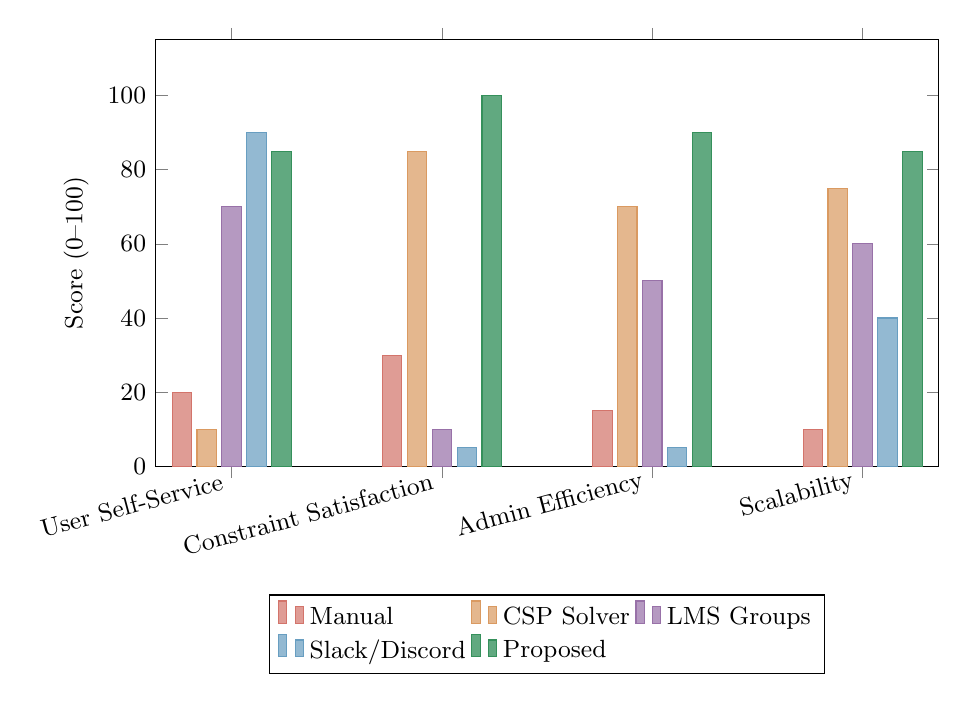
\begin{tikzpicture}
\begin{axis}[
    ybar,
    width=0.95\textwidth,
    height=7cm,
    ylabel={\small Score (0--100)},
    ylabel style={font=\small},
    symbolic x coords={User Self-Service, Constraint Satisfaction, Admin Efficiency, Scalability},
    xtick=data,
    x tick label style={font=\small, rotate=15, anchor=east},
    y tick label style={font=\small},
    bar width=7pt,
    ymin=0, ymax=115,
    enlarge x limits=0.12,
    legend style={at={(0.5,-0.3)}, anchor=north, font=\small, legend columns=3},
    legend cell align={left},
]
\addplot[fill=chartred!50, draw=chartred!70] coordinates {(User Self-Service,20) (Constraint Satisfaction,30) (Admin Efficiency,15) (Scalability,10)};
\addplot[fill=chartorange!50, draw=chartorange!70] coordinates {(User Self-Service,10) (Constraint Satisfaction,85) (Admin Efficiency,70) (Scalability,75)};
\addplot[fill=chartpurple!50, draw=chartpurple!70] coordinates {(User Self-Service,70) (Constraint Satisfaction,10) (Admin Efficiency,50) (Scalability,60)};
\addplot[fill=chartblue!50, draw=chartblue!70] coordinates {(User Self-Service,90) (Constraint Satisfaction,5) (Admin Efficiency,5) (Scalability,40)};
\addplot[fill=chartgreen!70, draw=chartgreen!90] coordinates {(User Self-Service,85) (Constraint Satisfaction,100) (Admin Efficiency,90) (Scalability,85)};
\legend{Manual, CSP Solver, LMS Groups, Slack/Discord, Proposed}
\end{axis}
\end{tikzpicture}
\caption{Quantitative comparison across four dimensions. The proposed system is the only approach achieving scores above 80 across all metrics simultaneously.}
\label{fig:comparison_chart}
\end{figure}

\subsection{Implementation Statistics}

Table~\ref{tab:metrics} summarizes the implementation characteristics.

\begin{table}[htbp]
\centering
\caption{Implementation Statistics}
\label{tab:metrics}
\small
\renewcommand{\arraystretch}{1.15}
\begin{tabular}{@{}ll@{}}
\toprule
\textbf{Metric} & \textbf{Value} \\
\midrule
Total TypeScript lines of code & 8,245 \\
Source files & 58 (31 TSX + 27 TS) \\
React components & 19 \\
API endpoints & 11 \\
Utility/library modules & 14 \\
Type definitions & 2 files (71+ types) \\
Framework & Next.js 16 (App Router) \\
Database & Firebase Firestore \\
Authentication & Firebase Auth + JWT \\
Hosting & Vercel (serverless) \\
Email service & Brevo (3-key round-robin) \\
\bottomrule
\end{tabular}
\end{table}

% ============================================================
\section{Discussion}
\label{sec:discussion}
% ============================================================

\subsection{Constraint Architecture Effectiveness}

The production deployment validates that real-time constraint enforcement is practically viable on serverless NoSQL infrastructure. The two-phase validation algorithm (Algorithms~\ref{alg:canAdd}--\ref{alg:validate}) achieves the critical balance: users retain full autonomy in member selection while the system guarantees 100\% constraint satisfaction for completed groups.

The progressive warning system proved effective in practice. Rather than imposing hard blocks early (which would frustrate users during the exploratory phase of group building), the system guides users toward constraint-satisfying compositions through timely warnings. This design respects human decision-making processes---users receive constraint status information at the point when it becomes actionable.

\subsection{NoSQL Integrity Without Transactions}

The six-layer data integrity framework demonstrates that comprehensive integrity guarantees are achievable on NoSQL infrastructure without relying on multi-document transactions. The key insight is that \textbf{defense-in-depth at the application level} can substitute for database-level transaction guarantees when the invariant set is known at design time.

The framework's effectiveness depends on two Firestore properties: (1)~strong consistency for single-document reads within the same request, which enables the read-before-write pattern for race-condition protection; and (2)~atomic single-document updates, which prevent partial-state issues during member operations. These properties are sufficient for our invariant set; applications requiring arbitrary cross-document invariants would need Firestore's multi-document transaction support or a relational database.

\subsection{Round-Robin in Practice}

The round-robin API key rotation handled the production deployment's peak load effectively. The registration burst (60\% of 823 users within 2 hours) generated approximately 500 OTP emails in a 2-hour window. With $n = 3$ keys, each key handled approximately 167 emails---well within the per-key burst capacity.

The stateless design proved advantageous: no coordination between serverless function instances was required, and cold-start counter resets had no observable impact on delivery. The primary trade-off is that load distribution is approximate rather than exact under cold starts, which is acceptable for this use case.

\subsection{Serverless Trade-offs}

The serverless architecture provides three significant advantages: zero-cost deployment on free tiers, automatic scaling, and zero operational maintenance. However, it introduces two trade-offs:

\begin{enumerate}[noitemsep,topsep=4pt]
    \item \textbf{In-memory state volatility:} The rate limiter and round-robin counter store state in server memory, which resets on cold starts. For the rate limiter, this means a brief window after cold start where rate limits are not enforced; for the round-robin counter, this means temporarily non-uniform key selection. Neither affects correctness---only best-effort quality.

    \item \textbf{Cold-start latency:} The first request after an idle period incurs cold-start overhead (typically 200--500ms on Vercel). This is acceptable for our use case where sub-second response times are sufficient, but would be problematic for latency-sensitive real-time applications.
\end{enumerate}

\subsection{Limitations}

\begin{enumerate}[noitemsep,topsep=4pt]
    \item \textbf{Cold-start problem:} Early registrants have fewer groups to browse; the platform is most effective when a critical mass of users has registered before group formation opens. The dual-gate system mitigates this.

    \item \textbf{In-memory rate limiting:} The current rate limiter does not persist across serverless function instances. For high-traffic deployments, a distributed store (e.g., Redis) would provide cross-instance persistence.

    \item \textbf{Constraint flexibility:} While the four-parameter model covers common diversity requirements, adding entirely new constraint \emph{types} (e.g., GPA distribution, schedule compatibility) requires code modifications.

    \item \textbf{Eventual consistency edge case:} While the read-before-write pattern prevents most race conditions, extremely rare simultaneous writes (within the same millisecond) could theoretically produce inconsistent state. This was not observed in production.

    \item \textbf{Single-deployment validation:} Production validation was performed at one organization. Multi-organization deployment studies are needed to validate generalizability.
\end{enumerate}

% ============================================================
\section{Future Work}
\label{sec:future}
% ============================================================

\begin{enumerate}[noitemsep,topsep=4pt]
    \item \textbf{Distributed rate limiting:} Replace the in-memory rate limiter with a Redis-backed implementation that persists across serverless function invocations and supports horizontal scaling. This would eliminate the cold-start rate-limit gap and enable consistent enforcement across multiple function instances.

    \item \textbf{Firestore transactions comparison:} Conduct a formal comparison between our application-level integrity framework and Firestore's native multi-document transactions, measuring the performance impact, developer complexity, and integrity guarantee trade-offs of each approach.

    \item \textbf{Constraint DSL:} Develop a domain-specific language allowing administrators to define arbitrary constraint rules (e.g., ``at most 2 from same subcategory AND GPA variance $< 0.5$'') via a web interface without code changes.

    \item \textbf{GraphQL API:} Extend the REST API with a GraphQL layer enabling fine-grained data fetching, reducing over-fetching on the browse interface, and enabling client-driven query composition for diverse frontend requirements.

    \item \textbf{Formal verification:} Apply model checking~\cite{baier2008} to verify the six-layer data integrity framework against a formal specification of the invariant set, providing machine-checked correctness guarantees beyond testing-based validation.

    \item \textbf{Multi-region deployment:} Extend the architecture for multi-region deployment with cross-region data replication, investigating the impact of geographic distribution on constraint enforcement latency and consistency guarantees.

    \item \textbf{Adaptive rate limiting:} Implement adaptive rate-limit policies that dynamically adjust thresholds based on observed traffic patterns, reducing false positives during legitimate bursts while maintaining protection against abuse.

    \item \textbf{Real-time constraint visualization:} Develop interactive constraint satisfaction visualizations showing users which group compositions are feasible given current membership, enabling more informed member selection.
\end{enumerate}

% ============================================================
\section{Conclusion}
\label{sec:conclusion}
% ============================================================

This paper presented a serverless web architecture for real-time constraint enforcement and multi-layer data integrity on NoSQL infrastructure. The core architectural innovations are:

A \textbf{formal constraint model} with four configurable parameters ($N$, $K$, $D$, $\mathcal{R}$), proven feasibility conditions (Theorem~\ref{thm:feasibility}), and a two-phase validation algorithm with correctness guarantee (Proposition~\ref{prop:correctness}) and $O(|T| + |\mathcal{R}|)$ time complexity.

A \textbf{six-layer data integrity framework} that enforces critical invariants---single-group membership, invite idempotency, duplicate prevention, and cascade cleanup---on NoSQL infrastructure without distributed locks or multi-document transactions, using defense-in-depth enforcement at the UI, API, and database-rule levels.

A \textbf{stateless round-robin API key rotation algorithm} with automatic failover that multiplies the effective throughput of rate-limited external APIs by a factor of~$n$, with $O(1)$ expected-time key selection, generalizable to any external service with per-key quotas.

A \textbf{five-layer defense-in-depth security architecture} providing robust authentication and authorization without institutional SSO dependency, combining OTP authentication, JWT sessions, database custom tokens, document-level access control, and IP-based sliding-window rate limiting.

Production deployment serving 823~users across 7~attribute categories validated the architecture with 100\%~constraint satisfaction for completed groups, zero data integrity violations across all concurrent operations, sub-second real-time feedback, and linear email-throughput scaling with API keys. The system operates at zero cost on serverless free tiers for deployments up to $\sim$1,000~users.

The architecture is domain-agnostic: any organization requiring constrained, self-service group formation can configure the constraint parameters, attribute categories, and composition rules without code changes. The complete implementation (8,245~lines of TypeScript, 58~files, 11~REST endpoints, 8~NoSQL collections) is available as open source at \url{https://github.com/harshaxyZ/idea.lab}.

% ============================================================
% Back Matter (Springer requirement)
% ============================================================

\section*{Acknowledgments}

The authors thank the Principal and Management of Don Bosco Institute of Technology, Bangalore, for their support and encouragement.

\section*{Declarations}

\begin{itemize}[noitemsep,topsep=3pt]
    \item \textbf{Funding:} This research received no external funding.
    \item \textbf{Conflict of interest:} The authors declare that they have no conflict of interest.
    \item \textbf{Ethics approval:} Not applicable. The study used anonymized, aggregate deployment data.
    \item \textbf{Consent to participate:} Not applicable.
    \item \textbf{Consent for publication:} Not applicable.
    \item \textbf{Data availability:} The source code and documentation are publicly available at \url{https://github.com/harshaxyZ/idea.lab}. The production deployment data (anonymized user statistics) are available from the corresponding author upon reasonable request.
    \item \textbf{Code availability:} Available at \url{https://github.com/harshaxyZ/idea.lab} under MIT license.
    \item \textbf{Author contribution:} All authors contributed to the study conception and design. Material preparation, data collection and analysis were performed by Mithun Gowda B and Harsha N. The first draft of the manuscript was written by Mithun Gowda B and all authors commented on previous versions of the manuscript. All authors read and approved the final manuscript.
\end{itemize}

\bibliographystyle{sn-basic-unsrt}
\bibliography{www-references}

\end{document}
